% RSS 2016 High Level Control of Modular Robots
%%%%%%%%%%%%%%%%%%%%%%%%%%%%%%%%%%%%%%%%%%%%%%%%%%%%%%%%%%%%%%%%%
%%%                    Included packages                 %%%
%%%%%%%%%%%%%%%%%%%%%%%%%%%%%%%%%%%%%%%%%%%%%%%%%%%%%%%%%%%%%%%%%

%%%  Included by IEEE:

\documentclass[conference]{IEEEtran}
\usepackage{times}

% numbers option provides compact numerical references in the text. 
\usepackage[numbers]{natbib}
\usepackage{multicol}
\usepackage[bookmarks=true]{hyperref}

%%%%%%%%%%%%%%%%%%%%%%%%%%%%%%%%%%%%%%%%%%%%%%%%%%%%%%%%%%%%%%%%%
%%%   Additional packages:

\usepackage{color}
\usepackage{mathtools}
\usepackage{amsmath} % assumes amsmath package installed
\usepackage{amssymb}  % assumes amsmath package installed
%\usepackage[final]{pdfpages} % for including pdfs
\usepackage{subcaption}
\usepackage{multirow}
\usepackage{float}
\usepackage{amsmath}
\usepackage{nccmath} % for fleqn
\usepackage{algorithm}

%%%%%%%%%%%%%%%%%%%%%%%%%%%%%%%%%%%%%%%%%%%%%%%%%%%%%%%%%%%%%%%%%
%%%  Macros:

% For making things invisible during double-blind review. Put "#1" in the
% the braces to make the text appear later.:
\newcommand{\doubleBlind}[1]{} 

% For marking Todos and changes
\newcommand{\TODO}[1]{ {\bf \textcolor{red}{TODO:} #1 }}
\newcommand{\abj}[1]{\textcolor{blue}{#1}}
\newcommand{\dbj}[1]{\textcolor{blue}{\sout{#1}}}
\newcommand{\cbj}[2]{\textcolor{blue}{\sout{#1}}\textcolor{blue}{~#2}}
\newcommand{\abt}[1]{\textcolor{magenta}{#1}}
% Handy commands
\newcommand{\lt}{{\tt True }}
\newcommand{\lf}{{\tt False }}
\newcommand{\ltnsp}{{\tt True}}
\newcommand{\lfnsp}{{\tt False}}
\newtheorem{definition}{Definition}
\DeclareMathOperator{\F}{\rotatebox[origin=c]{45}{$\Box$}}
\DeclareMathOperator{\X}{\bigcirc}
\DeclareMathOperator{\G}{\Box}
\newcommand{\LTLG}{\G}
\newcommand{\LTLF}{\F}
\newcommand{\LTLX}{\X}

\newfloat{spec}{thb}{lop} %{thb}{lop}
\floatname{spec}{Specification}
\makeatletter
\newcommand{\leqnomode}{\tagsleft@true}
\newcommand{\reqnomode}{\tagsleft@false}
\makeatother
%%%%%%%%%%%%%%%%%%%%%%%%%%%%%%%%%%%%%%%%%%%%%%%%%%%%%%%%%%%%%%%%%

\pdfinfo{
   /Author (Mystery Authors)
   /Title  () %TODO add title
   /CreationDate ()
   /Subject ()
   /Keywords ()
}

%%%%%%%%%%%%%%%%%%%%%%%%%%%%%%%%%%%%%%%%%%%%%%%%%%%%%%%%%%%%%%%%
%%%                     Main document                        %%%
%%%%%%%%%%%%%%%%%%%%%%%%%%%%%%%%%%%%%%%%%%%%%%%%%%%%%%%%%%%%%%%%
\usepackage{graphicx}

\begin{document}


\title{An Integrated System for Autonomously Performing Perception-Driven Tasks with Modular Robots}

\author{Mystery Authors}

% \author{\authorblockN{Gangyuan Jing}
% \authorblockA{
% Cornell University\\
% \texttt{gj56@cornell.edu}}
% \and
% \authorblockN{Tarik Tosun}
% \authorblockA{Univ. of Pennsylvania\\
% \texttt{tarikt@grasp.upenn.edu}}
% \and
% \authorblockN{Mark Yim}
% \authorblockA{Univ. of Pennsylvania\\
% \texttt{yim@grasp.upenn.edu}}
% \and
% \authorblockN{Hadas Kress-Gazit}
% \authorblockA{Cornell University\\
% \texttt{hadaskg@cornell.edu}}
% }

\maketitle

\begin{abstract}

We present a fully autonomous modular robot system that can perform complex, high-level tasks in an unknown environment without external sensing or control. The validity of the system is demonstrated in a real-world experiment. The physical robot is composed of modules that support multiple robot configurations. An onboard 3D sensor provides information about the environment, which is used to perform SLAM in the unknown environment and inform exploration and feedback control. No external sensors, pose providers, or beacons are used. A centralized planning algorithm uses the information from the environment and the desired high-level task description to synthesize low-level controllers to perform locomotion, reconfiguration, and special actions. A novel, centralized, self-reconfiguration method is used to change robot configurations when desired. To the authors' knowledge, the proposed work comprises the first modular robot system that uses perception-driven reconfiguration to intelligently adapt to an \textit{a priori} unknown environment to perform complex tasks.

\end{abstract}

\IEEEpeerreviewmaketitle

       %     ____      __                 __           __  _
       %    /  _/___  / /__________  ____/ /_  _______/ /_(_)___  ____
       %    / // __ \/ __/ ___/ __ \/ __  / / / / ___/ __/ / __ \/ __ \
       %  _/ // / / / /_/ /  / /_/ / /_/ / /_/ / /__/ /_/ / /_/ / / / /
       % /___/_/ /_/\__/_/   \____/\__,_/\__,_/\___/\__/_/\____/_/ /_/

\section{Introduction} \label{sec:introduction}
%
Modular self-reconfigurable robot (MSRR) systems are composed of a number of simple repeated robot elements (called \emph{modules}) that connect together to form larger robotic structures. These systems can \emph{self-reconfigure}, changing their shape (\emph{i.e.} the connective structure of the modules) to meet the needs of the task at hand.
In principal, these systems can address a wide variety of tasks by transforming into a wide variety of morphologies.   

Over the past three decades, dozens of modular robot systems have been built \cite{Yim2007a}. Existing literature provides ample evidence of MSRR systems reconfiguring and assuming interesting morphologies, as well as methods for programming, controlling, and simulating modular robots \cite{Yim2007,Jing2016,Yim1994}.

These capabilities are impressive, and each represents a significant research accomplishment in its own right. However, in order to truly live up to their promise of flexible capability in the real world, MSRR systems must demonstrate autonomy: moving, navigating, interacting with objects, and self-reconfiguring, all in unknown environments and without external localization or control. 

We provide a system capable of \emph{autonomously} solving \emph{high-level
tasks} in \emph{unknown environments} using \emph{modular self-reconfigurable
robots}.  A \emph{high-level task} is specified in terms
of general objectives, and requires some decision-making regarding the specific
way in which the task will be solved. The environment is \emph{unknown}, meaning
that the robot does not have a map of the environment or obstacles before the
task begins. To our knowledge, this paper represents the first example of a truly autonomous MSRR system accomplishing these kinds of tasks.

The system we present provides four major tools:

\begin{enumerate}
\item \textbf{Hardware:} The SMORES-EP Modular robot, and sensing hardware designed
to work with SMORES-EP.  
\item \textbf{High-Level Task Description:} A framework for specifying high-level
tasks in terms of state machines, and for abstracting modular robots.
\item \textbf{Perception and Environment Characterization:} Tools for SLAM,
navigation, and obstacle avoidance with modular robots, as well as tools that
parse sensor information into actionable conclusions relevant to high-level
tasks.
\item \textbf{Reconfiguration:} Software and hardware tools enabling robust
autonomous reconfiguration with SMORES-EP.
\end{enumerate}

Through hardware experiments, we demonstrate that this system is capable of autonomously completing high-level object-retrieval tasks in unknown environments.

%
%    _____            __                    ____                        _
%   / ___/__  _______/ /____  ____ ___     / __ \_   _____  ______   __(_)__ _      __
%   \__ \/ / / / ___/ __/ _ \/ __ `__ \   / / / / | / / _ \/ ___/ | / / / _ \ | /| / /
%  ___/ / /_/ (__  ) /_/  __/ / / / / /  / /_/ /| |/ /  __/ /   | |/ / /  __/ |/ |/ /
% /____/\__, /____/\__/\___/_/ /_/ /_/   \____/ |___/\___/_/    |___/_/\___/|__/|__/
%      /____/
\subsection{System Overview}
%
Here we provide a brief overview of the entire system.  Figure~\ref{fig:overview} shows a flowchart which serves as a visual companion to this section. 

Tasks are specified in a high-level mission planner using Linear Temporal Logic (LTL). The user does not specify a specific sequence of actions that should be completed, but rather expresses the task in the form of logical statements which map conditions to actions. Additionally, because a modular robot system is being used to complete the task, the task definitions do not directly specify which configuration (connected robot shape) should be used to execute each action. Instead, actions are specified in an abstract sense, for example ``If you encounter a pink object, pick it up." When a pink object is encountered, the planner will evaluate the environment surrounding the pink object and decide whether the current configuration of the robot is capable of executing a "pick up" action.  If it is not, the planner may decide reconfigure to another configuration which is capable of picking up the object under the current conditions.  Section \ref{sec:high-level} describes our high-level mission planner in detail.

Our system is built around the SMORES-EP modular robot system, described in detail in Section \ref{sec:hardware}. Because SMORES-EP is capable of changing its physical morphology through self-reconfiguration, we must provide appropriate high-level abstractions of the robot that allows our high-level planner to address tasks.  These abstractions are described in Section \ref{sec:configuration-specifics}.

The modularity of our robot makes sensing challenging.  We have extended the existing SMORES-EP robot system by developing a sensor module which can be carried as part of a cluster of SMORES-EP modules to provide sensing and localization information, described in detail in Section \ref{sec:sensor_module}.

Our system is intended to address tasks where the robot is required to explore an \emph{a priori} unknown environment and react to what it encounters.  To that end, we provide a suite of software tools for sensing and perception. Our perception tools allow a SMORES-EP robot to perform SLAM, navigation, and obstacle avoidance using the sensor module.  This software has been specifically optimized to work with data from the onbord XTion Pro depth camera, and to run efficiently using the limited computation power of the onboard UPboard computer.  Additionally, a novel next-best-view algorithm automatically selects waypoints in the environment to allow the robot to maximize information gain as it explores.  These tools are discussed in detail in Section \ref{sec:perception}

While exploring, the robot must recognize and react to objects and features of the environment.  We provide environment characterization tools that parse raw sensor information into actionable conclusions relevant to high-level tasks.  More specifically, we provide classifiers that can identify objects based on color, and classifiers that characterize different kinds of environments (such as ledges and tunnels) based on 3D depth information.  These are described in Section \ref{sec:environment-characterization}.

Finally, we provide software and hardware tools enabling rapid, robust, autonomous reconfiguration with SMORES-EP. Our system is capable of completing reconfiguration tasks without any external localization, by using AprilTags for reconfiguration. The system features an overhead camera carried along with the robot as part of the sensor module, which is a novel localization modality for reconfiguration. Our reconfiguration system also relies on elements of our perception algorithms, which provide goal pose information for docking.  Our reconfiguration tools are described in Section \ref{sec:reconfiguration}.

After presenting the complete system, we demonstrate how these individual components form a complete system capable of autonomously solving high-level tasks in unknown environments with modular robots.  In Section~\ref{sec:experiments}, we show how our system can be used to complete a realistic object retrieval task in an unknown environment with full autonomy.  Finally, in Section~\ref{sec:discussion}, we evaluate the success of our system in achieving its goals, and conclude.
%
% System Overview Figure
\begin{figure}
\begin{center}
\includegraphics[width=0.4\textwidth]{images/overview.png}
\caption{System Overview Flowchart}
\label{fig:overview}
\end{center}
\end{figure} 
%
%     ____       __      __           __   _       __           __
%    / __ \___  / /___ _/ /____  ____/ /  | |     / /___  _____/ /__
%   / /_/ / _ \/ / __ `/ __/ _ \/ __  /   | | /| / / __ \/ ___/ //_/
%  / _, _/  __/ / /_/ / /_/  __/ /_/ /    | |/ |/ / /_/ / /  / ,<
% /_/ |_|\___/_/\__,_/\__/\___/\__,_/     |__/|__/\____/_/  /_/|_|

\section{Related Work}\label{sec:related-work}
\subsection{Autonomous Self-Reconfiguration}
\label{autonomous-self-reconfiguration}
%
Autonomous reconfiguration has been demonstrated with several modular robot systems. CKbot, Conro, and MTRAN have all demonstrated the ability to join disconnected clusters of modules together \cite{Yim2007, Rubenstein2004,Murata2006}. In order to align, Conro uses infra-red sensors on the docking faces of the modules, while CKBot and MTRAN use a separate sensor module on each cluster.  In all cases, individual clusters locate and servo towards each other until they are close enough to dock.

While these proof-of-concept experiments demonstrate the ability to reconfigure, these capabilities have not been used as part of a larger system to complete tasks. The experiments do not include any planning or sequencing of multiple reconfiguration actions in order to create a goal structure appropriate for a task.  Additionally, because these are all chain-type modular robots, individual modules are not able to locomote on their own, and mobile clusters of modules are limited to slow crawling gaits.  Consequently, reconfiguration is very time consuming, with a single connection requiring 5-15 minutes.

Other work has focused on reconfiguration planning, but not autonomous reconfiguration.  Paulos et al. present a system in which self-reconfigurable modular boats self-assemble into functional floating structures, such as a bridge \cite{Paulos2015}.  Like the SMORES-EP modules used in this paper, individual boat modules are able to move about the pool, allowing for rapid reconfiguration.  However, external localization is provided by an overhead AprilTag system. 

To our knowledge, this paper represents the first examples of a MSRR system autonomously making the decision to reconfigure in response to its sensed environment, and then actually reconfiguring\ in order to complete its task.  In \cite{Dorigo2013}, hand-bot and foot-bot elements of the swarmanoid system connect and disconnect in order to complete a book-retrieval task, but the decision to take this action is not made autonomously by the robot in response to sensed environment conditions.
%
\subsection{Modular Robots Completing Tasks}
%
%%% Paragraph from intro
% The traditional approach to achieving flexible
% robots is to build  monolithic systems that are highly capable, but also highly
% complex (\emph{e.g.} large humanoids).  Self-reconfigurability is an elegant,
% scalable alternative: since the shape of the robot is not fixed, each individual
% task can be solved with a morphology that is only as complicated as it needs
% to be.
%%%
Modular robots have long been regarded as having the potential to make impact in unknown environments (such as search and rescue scenarios), because  self-reconfiguration theoretically gives them the flexibility to respond to whatever they encounter \cite{Yim2007a,Yim2000}.  However, examples of MSRR actually operating in unknown environments are very limited. To our knowledge, no MSRR system has been used for SLAM. We believe our system has more autonomy in an unknown environment than any existing modular robot system, and represents an important step toward the application of MSRR in the real world.

MSRR systems have demonstrated the ability to accomplish low-level tasks such as various modes of locomotion \cite{Yim1994}. Recently work includes a system which integrate many low-level capabilities of a MSRR system in a design library, and accomplishes high-level user-specified tasks by synthesizing elements of the library into a reactive state-machine \cite{Jing2016}. While this system demonstrates autonomy with respect to task-related decision making, it is designed to operate in a fully known environment with external sensing.

There is work on mapping with swarm robot systems. The Millibot system has demonstrated the ability to map a partially unknown environment when operating as a swarm \cite{Grabowski2000}. The autonomy of the Millibot swarm is limited: a human operator makes all high-level decisions, and is responsible for navigation using a GUI. Certain members of the swarm are designated as ``beacons,'' and have known locations, making the environment only partially unknown.

The swarm-bots are a MSRR system that has been applied in exploration \cite{Dorigo2005} and collective manipulation \cite{Mondada2005} scenarios.  Like the Millibots, exploration is demonstrated in partially unknown environments, with some members of the swarm acting as ``beacons'' with known location.  In a collective manipulation task, the swarm-bots have limited autonomy, with a human operator specifying the location of the manipulation target and the global sequence of manipulation actions. The swarmanoid project (successor to the swarm-bots), moves a step beyond this capability, using a heterogeneous swarm of ground and flying robots (called ``hand-'', ``foot-'', and ``eye-'' bots) to perform exploration and object retrieval tasks in unknown environments \cite{Dorigo2013}.  However, there is no reconfiguration or other transformation of the robots to adapt to unknown features of the environment. Although the location of the object to be retrieved is unknown, the method for retrieving the object is known and constant. We utilize the self-reconfiguration capability of MSRR systems to take autonomy a step further. The system uses perception of the environment to drive not only exploration but also the choice of robot configuration. This allows the robot to adapt its abilities to surmount challenges arising from \textit{a priori} unknown features in the environment.

%     __  __               __
%    / / / /___ __________/ /      ______ _________
%   / /_/ / __ `/ ___/ __  / | /| / / __ `/ ___/ _ \
%  / __  / /_/ / /  / /_/ /| |/ |/ / /_/ / /  /  __/
% /_/ /_/\__,_/_/   \__,_/ |__/|__/\__,_/_/   \___/

\section{Hardware} % (fold)
\label{sec:hardware}
%
\subsection{SMORES-EP Modular Robot} \label{sec:smores}
%
Our system is built around the SMORES-EP robot, but could easily be adapted to
work with other hardware platforms.  In this section, we provide a brief
introduction to the technical capabilities of SMORES-EP.

Each module is about the size of an \textit{80mm cube}, and has four actuated DoF - three continuously rotating faces (left, right, and
pan)  and one central hinge (tilt) with a \(180^\circ\) range of motion
(Fig.~\ref{fig:smores-module}). The DoF marked left, right, and tilt  have
 axes of rotation that are parallel and coincident. A single module can use its
left and right wheels to drive around as a two-wheel differential drive robot.
All four faces of the SMORES-EP module have electro-permanent (EP) magnets
that serve as a high-strength, low-energy connector for self-reconfiguration
\cite{tosun2016design}.  Any face of one module can connect to any face of
another.

The magnetic connectors can also attach to objects made of ferromagnetic
materials (such as steel).  By taking advantage of this capability, SMORES-EP
modules can use their magnets to attract, lift, and carry metal objects.
Provided the attachment surface is flat and smooth, the attachment force
between a SMORES-EP face and a strongly ferromagnetic object can be as high as
90N \cite{tosun2016design}.

Each module has an onboard battery, microcontroller, and 802.11b wireless
module to send and receive UDP packets.  In this work, clusters of SMORES
modules were controlled by a central computer running a Python program that
sends wireless commands to control the four DoF and magnets of each module.
Battery life is about one hour (depending on motor, magnet, and radio usage),
and commands to a single module can be received at a rate of about 20hz.
Wireless networking was provided by a standard off-the-shelf  router, with a
range of about 100 feet.
\TODO{Mention dummy modules.}
%% SMORES-EP module DoF picture
\begin{figure}   
\begin{center}
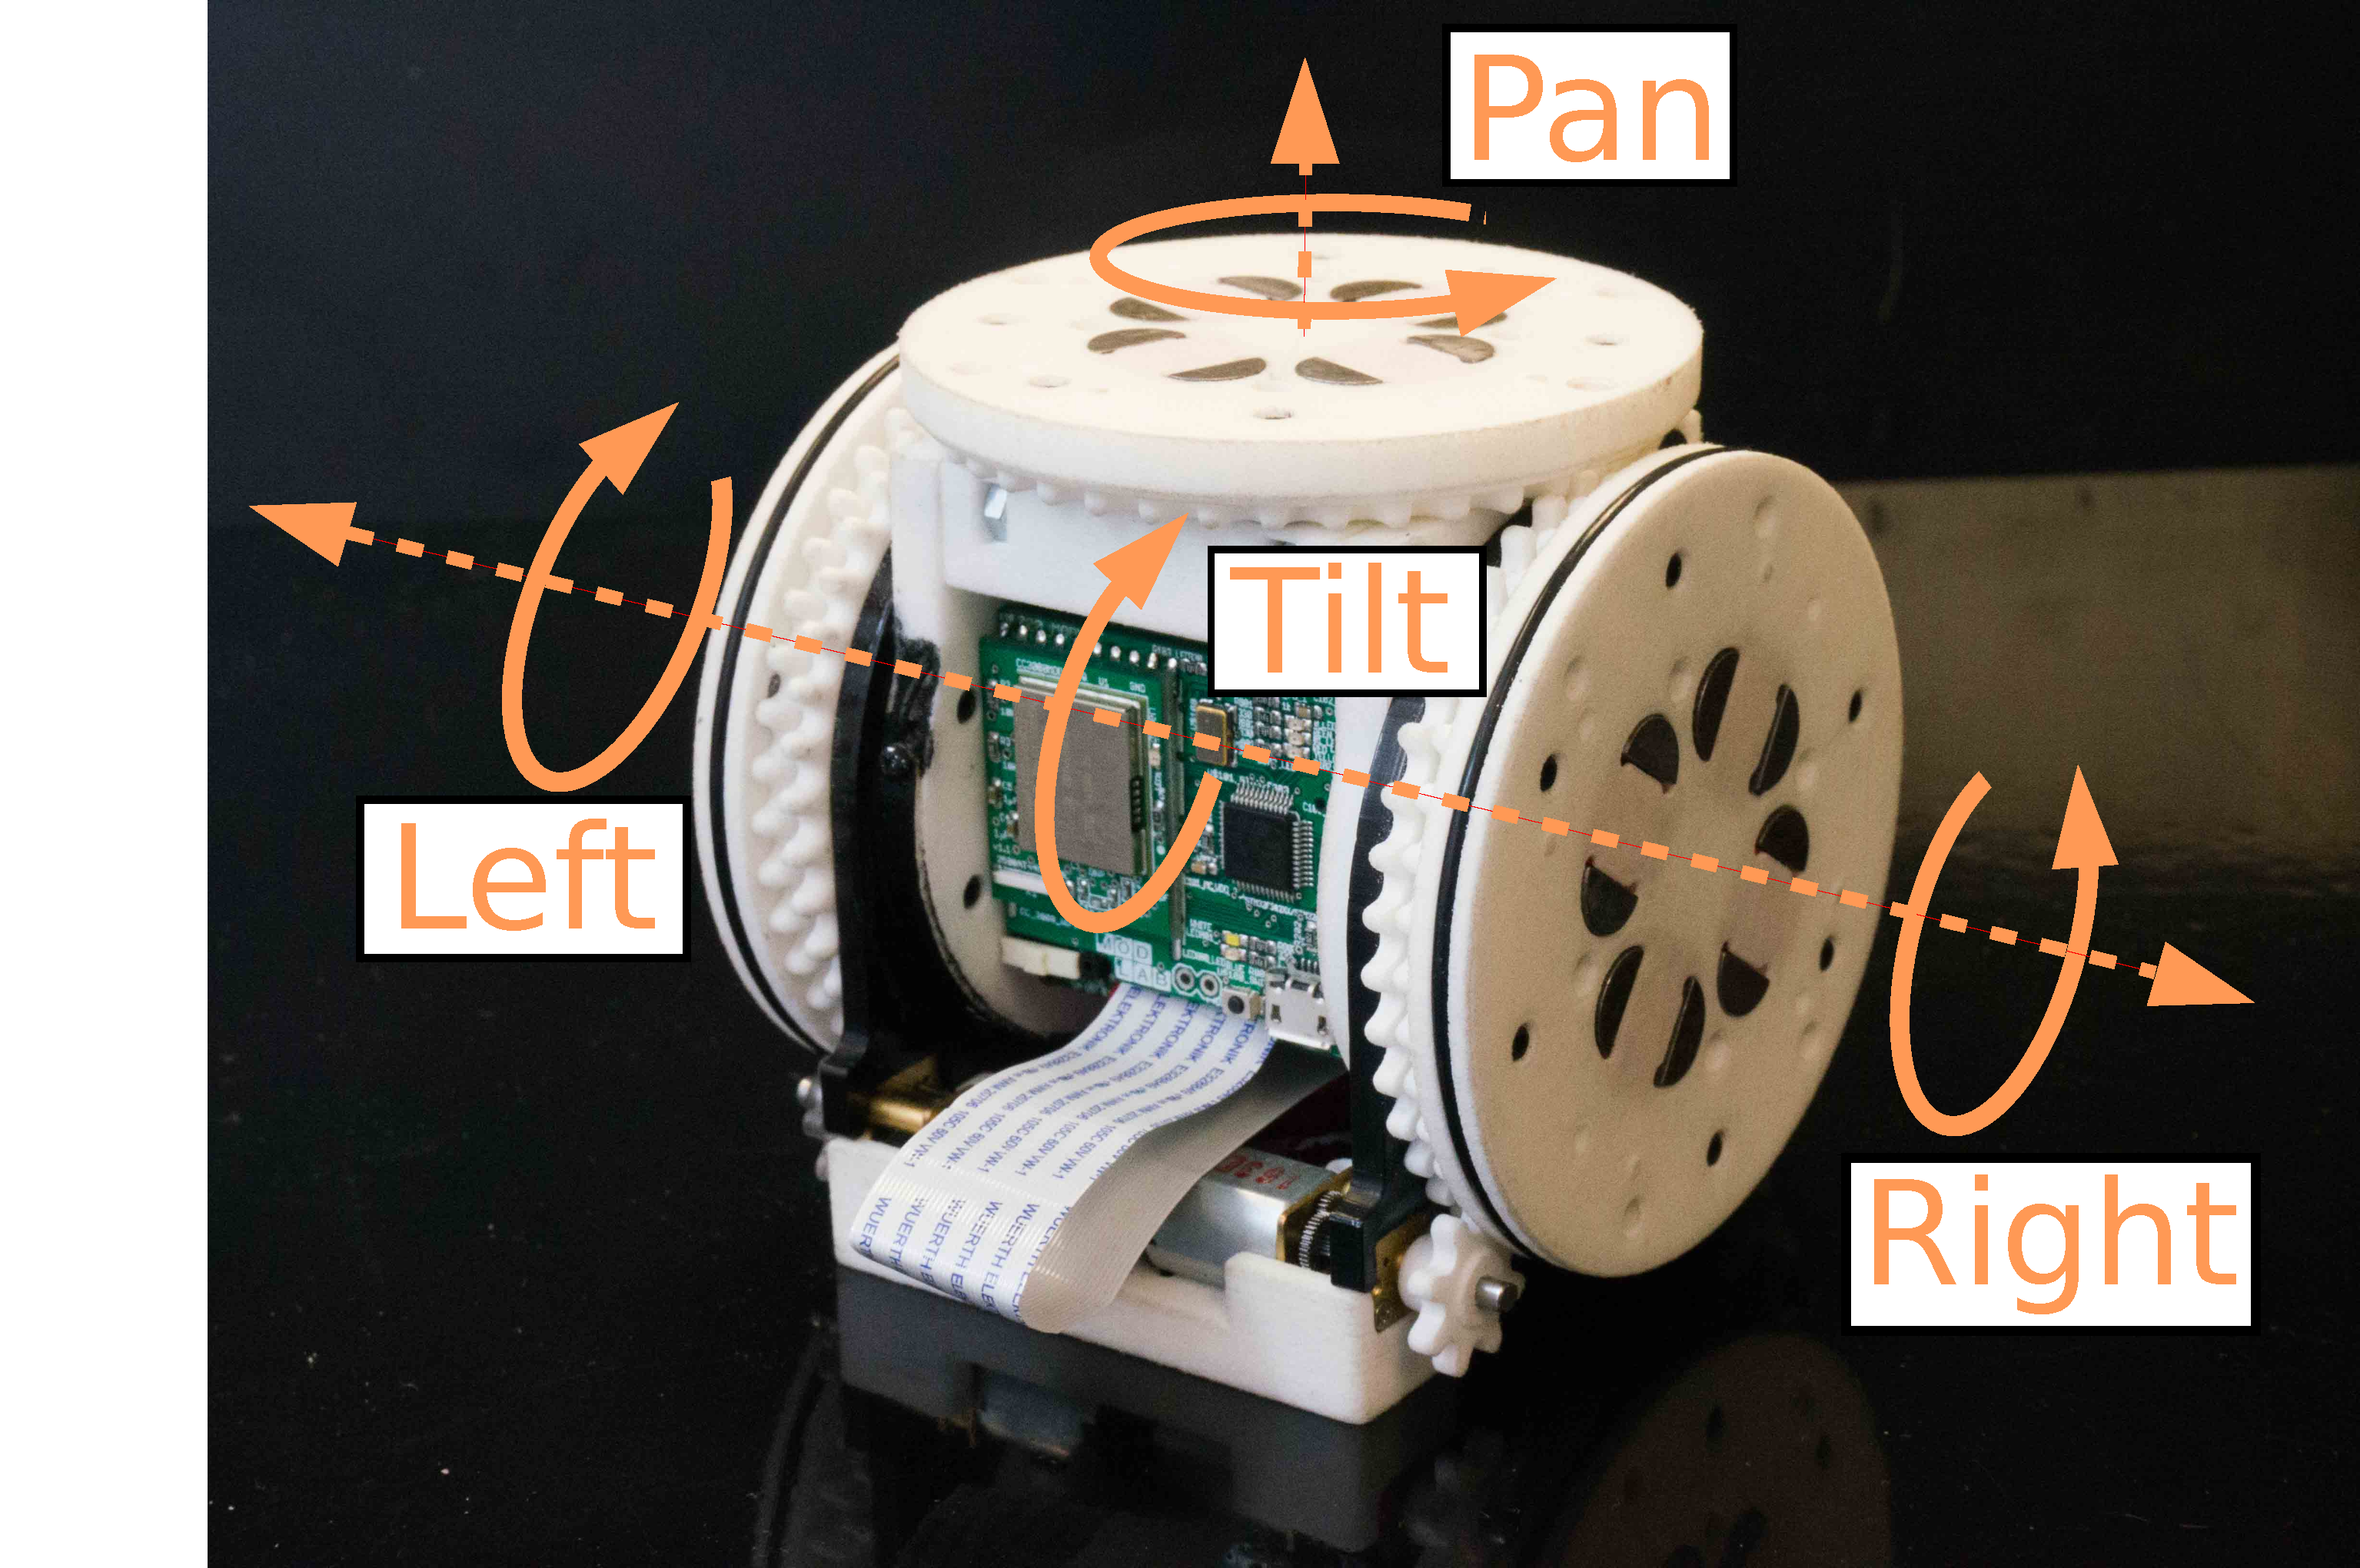
\includegraphics[height=1.5in]{images/smores_dof.pdf}
\end{center}
\caption{SMORES-EP module}
\label{fig:smores-module}
\end{figure}
%

\subsection{Sensor Module} % (fold)
\label{sec:sensor_module}
%

In MSRR systems, sensing and processing capabilities of individual modules are severely limited by the size and weight constraints of the module form factor. Therefore, the proposed system uses a special sensor module dedicated to sensing and processing equipment, shown in Figure \ref{fig:sensor-module}. The module has no actuation capabilities and is larger than SMORES-EP modules. It is equipped with a front-facing Xtion Pro Live RGB-D sensor which enables the robot to explore and map the environment and recognize objects of interest. A high, downward-facing HD webcam is included to provide a view of the robot itself, which is used for self-reconfiguration. Finally, an UP computing board provides high performance I/O and processing capability in a small form factor. The UP Board used in the proposed system has an Intel Atom 1.92 GHz processor, 4 GB memory, and a 64 GB hard drive. It is network connected via 802.11 wifi. A battery provides power to the Up Board with a lifetime of about 1.5 hours.

% Sensor Module Figure
\begin{figure}
\begin{center}
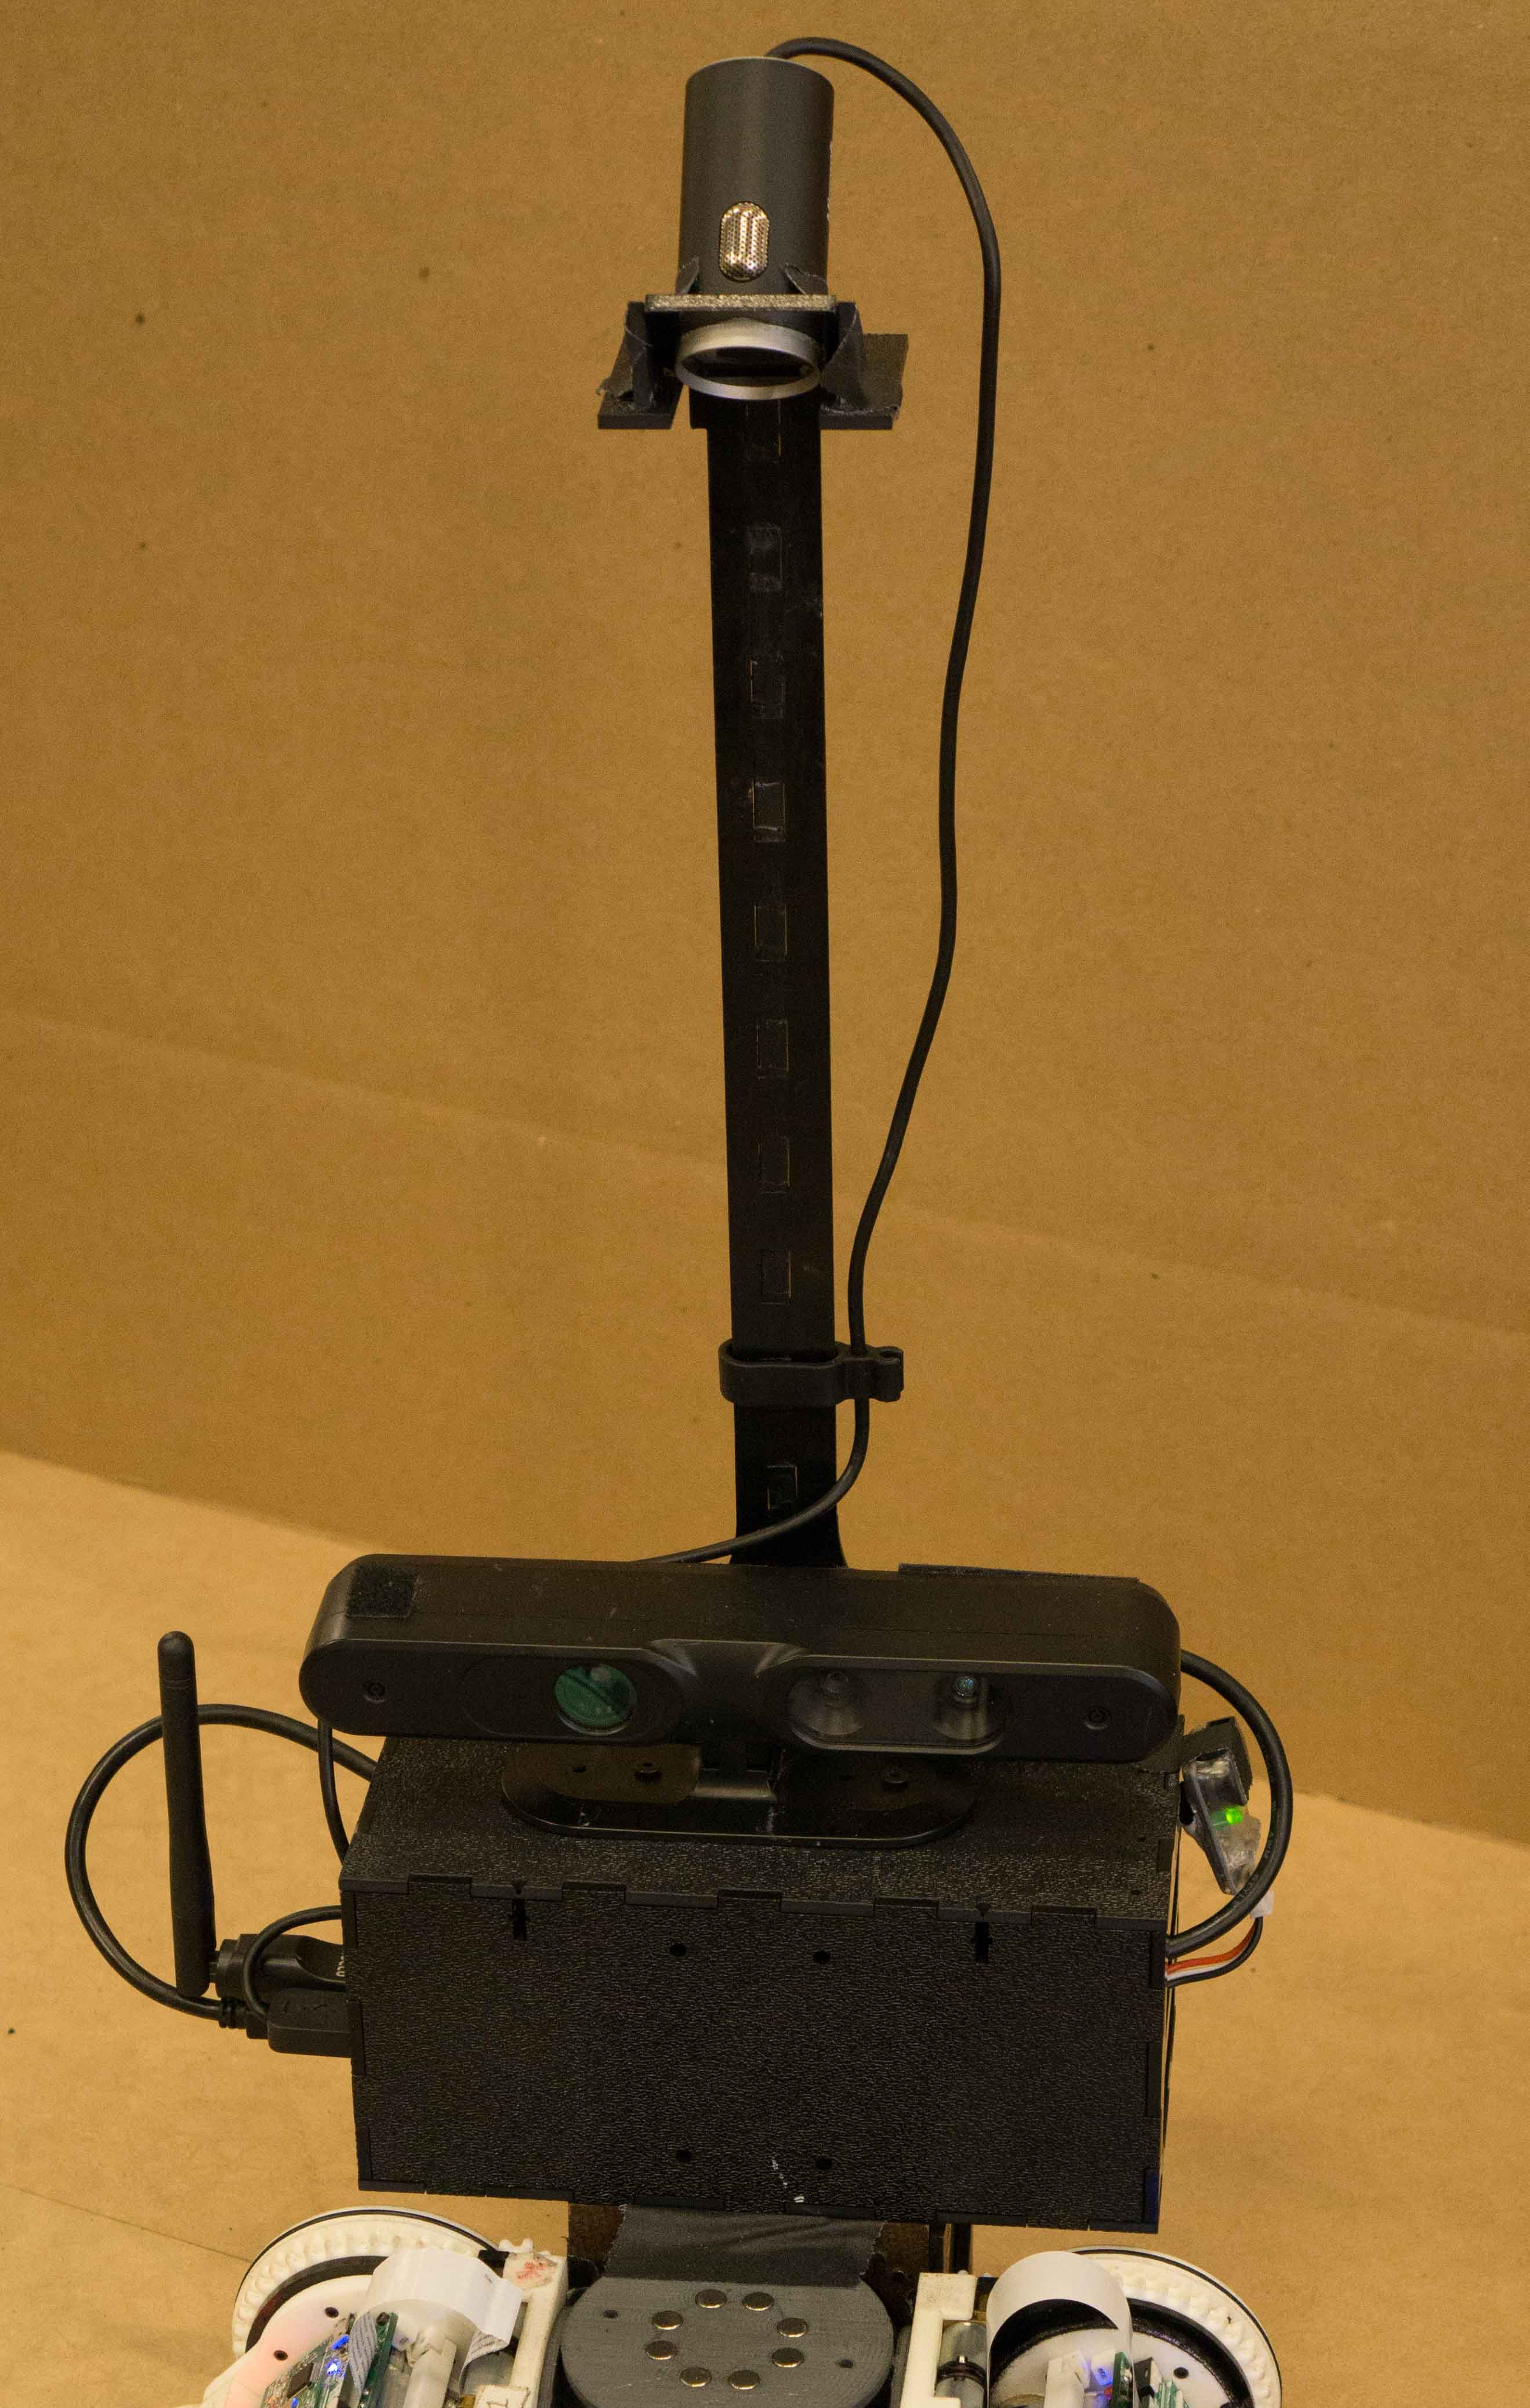
\includegraphics[width=0.3\textwidth]{images/sensor_module.jpg}
\caption{Sensor module.}
\label{fig:sensor-module}
\end{center}
\end{figure}

%
% subsection sensor_module (end)
% section hardware (end)
%

%     ____                            __  _
%    / __ \___  _____________  ____  / /_(_)___  ____
%   / /_/ / _ \/ ___/ ___/ _ \/ __ \/ __/ / __ \/ __ \
%  / ____/  __/ /  / /__/  __/ /_/ / /_/ / /_/ / / / /
% /_/    \___/_/   \___/\___/ .___/\__/_/\____/_/ /_/
%                          /_/
\section{Perception and Environment Characterization}
\label{sec:perception-and-env-characterization}
%
Since the proposed system performs tasks in unknown environments and conditions, a robust suite of perception algorithms is required to inform control and decision-making. The robot must have the ability to explore and build a map of its environment while avoiding obstacles and tracking its pose. The system must be able to recognize objects and regions of interest related to the desired task. Finally, the system must characterize the environment in terms of configuration capabilities. Features in the environment may restrict which robot configurations can viably perform parts of the high-level task, such as retrieving an object or navigating to a waypoint. The system needs to recognize these features to be able to intelligently choose the appropriate robot configuration for performing the task.

\subsection{Perception}
\label{sec:perception}
%
To facilitate the use of open source software and enable networking between components, the proposed system is built in a ROS framework.\footnote{http://www.ros.org} Robot pose is provided by a RGB-D SLAM software package called RTAB-MAP\cite{rtabmap}. A 3D map of the environment is incrementally built and stored in an efficient octree-based volumetric map using Octomap\cite{octomap}.  Task-related objects and regions of interest in the environment are given distinctive colors. These colors are recognized using color recognition software\footnote{CMVision: http://www.cs.cmu.edu/$\sim$jbruce/cmvision/} and tracked in 3D using depth information from the Xtion sensor.\footnote{Lucas Coelho Figueiredo: https://github.com/lucascoelho91/ballFollower}

The system must explore the \textit{a priori} unknown environment to search for task-related objects and zones. The system performs this exploration in an intelligent manner using a new next best view planner for object exploration created by two of the authors.\footnote{This work has been newly accepted for journal publication in 2017}. The exploration algorithm uses the current volumetric map of the environment and estimates the next reachable sensor viewpoint that will observe the largest volume of undiscovered portions of objects. It also estimates the amount of information (in an entropy-reduction sense) that will be gained from a sensor measurement taken at that viewpoint. To integrate into the proposed system, the exploration algorithm is offered as a service that can be queried by the high-level planner when desired. A volumetric map of the environment and the reachable space of sensor viewpoints in that map must be provided to the algorithm. Note that the reachable space is dependent on the locomotion capabilities of the specific robot configuration. The algorithm then computes and returns the next best view for the sensor, which the high-level planner can then set as a navigation waypoint.

\begin{figure}[t]
      \centering
      \begin{subfigure}[t]{0.15\textwidth}
        \includegraphics[width=\textwidth]{images/free.png}
        %\label{fig:obja}
        \caption{\textbf{``free'}' environment}
    \end{subfigure}
    \begin{subfigure}[t]{0.15\textwidth}
        \includegraphics[width=\textwidth]{images/ledge.png}
        %\label{fig:objb}
        \caption{\textbf{``ledge''} environment}
    \end{subfigure}
        \begin{subfigure}[t]{0.15\textwidth}
        \includegraphics[width=\textwidth]{images/tunnel.png}
        %\label{fig:objb}
        \caption{\textbf{``tunnel''} environment}
    \end{subfigure}
      \caption{Environment characterization types for object retrieval.}
      \label{fig:characters}
   \end{figure}


\subsection{Environment Characterization}
\label{sec:environment-characterization}
%
In order to intelligently choose appropriate configurations when performing tasks, the robot must perceive and characterize its environment into a discrete set of environment types that correspond with configuration capabilities. The proposed system includes a perception component that discretely characterizes the environment for the purpose of retrieving an object. This characterization can then be used by the high-level planner to determine the appropriate configuration and gait for successful object retrieval. The 3 environment characterizations are shown in Figure \ref{fig:characters}. The environment surrounding objects to be retrieved is assumed to fall under one of these types. If the object's position is higher than a threshold height, the environment is characterized as the ``ledge'' environment. This requires a configuration/gait that can reach up to the top of the ledge to retrieve the object. If the object is on the ground, the remaining two characterizations are distinguished using the following method, illustrated in Figure \ref{fig:characterization}. An occupancy grid is created around the object, and all grid cells within a robot radius of obstacles are denoted unreachable (light blue in Figure \ref{fig:characterization}). The closest reachable point to the object within $20^o$ of the robot's line of sight to the object is selected. If the distance from this point to the object is greater than a threshold value, the environment is characterized as ``tunnel''. To retrieve the object in this type of environment, a configuration with a long, thin arm is required to reach between the surrounding obstacles to retrieve the object. If the distance to the object is under the threshold, the environment is characterized as ``free''. This means no special configurations are required to reach the object. If the environment type is ``tunnel'', the algorithm also selects a navigation waypoint at which the robot can reconfigure before retrieving the object. This waypoint is calculated by extending the closest point farther away from the object to be retrieved (red arrow in Figure \ref{fig:characterization}). This information is passed to the high-level planner for use in controller synthesis.

% Characterization method
\begin{figure}
\begin{center}
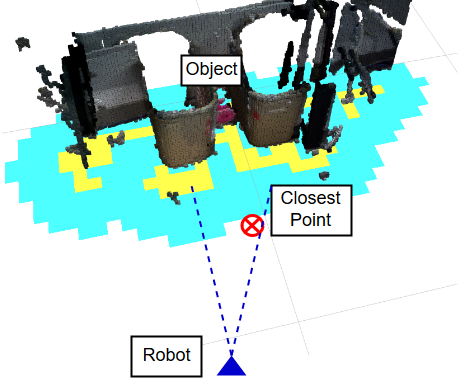
\includegraphics[width=0.4\textwidth]{images/characterization.png}
\caption{\textbf{Tunnel} environment characterization method.}
\label{fig:characterization}
\end{center}
\end{figure}


%    ______            _____          _____                 _ _____
%   / ____/___  ____  / __(_)___ _   / ___/____  ___  _____(_) __(_)_________
%  / /   / __ \/ __ \/ /_/ / __ `/   \__ \/ __ \/ _ \/ ___/ / /_/ / ___/ ___/
% / /___/ /_/ / / / / __/ / /_/ /   ___/ / /_/ /  __/ /__/ / __/ / /__(__  )
% \____/\____/_/ /_/_/ /_/\__, /   /____/ .___/\___/\___/_/_/ /_/\___/____/
%                        /____/        /_/
\section{Configuration-Specific Controllers}
\label{sec:configuration-specifics}
Modular robots can change their configurations to gain new capabilities and accomplish various tasks.
Since the configuration affects the dynamics of the modular robots, configuration-specific controllers are required for commanding modular robots.
In this work, we utilize a library-driven system to create, organize and execute modular robot behaviors based on the robot configuration, the runtime environment and the robot behavior properties.
A modular robot behavior library consists of a collection of different library entries.
A library entry is defined as $l = (C,B_C,P_e,P_b)$ where:
\begin{itemize}
\item $C$ specifies the configuration of the robot
\item $B$ is the controller that commands the robot to perform a specific behavior
\item $P_e$ holds information about the environment where this library entry is suitable
\item $P_b$ describes the properties of the robot behavior
\end{itemize}

In order to control the robot to perform desired behaviors in the \textit{a priori} unknown environment, we employ a perception-driven method to intelligently choose the library entry from the modular robot behavior library.
First the desired behavior is specified as a set of behavior properties $P'_b$.
We characterize the current environment as described in Section~\ref{sec:environment-characterization} to a set of environment properties $P'_e$.
Then we can find a set of library entries that match with $P'_e$ and $P'_b$.
If a library entry requires a different configuration from the current robot configuration, a reconfiguration process can be performed as described in Section~\ref{sec:reconfiguration}.
To minimize complexity in runtime, we bias towards the library entries that require no reconfiguration when choosing the appropriate library entry.
Once the library entry is selected, the controller $B$ is executed to produce the desired robot behavior.

In this work, we created five library entries for two different configurations as listed in Table.~\ref{table:1}. 
The ``Tank'' configuration shown in Fig.~\ref{fig:dropoff} is capable of picking up and dropping items in ``free'' environment while driving on a flat plain as a holonomic drive robot.
The ``Proboscis'' configuration shown in Fig.~\ref{fig:pink_grab} is setup to have a long arm for reaching between obstacles in a ``tunnel'' environment to grasp objects. However, the locomotion ability of this configuration is limited to forward/backward motion, making it unsuitable for general navigation.

\begin{table}
\centering
\begin{tabular}{ |c|c|c| } 
 \hline
 \multirow{2}{6em}{Configuration} & Behavior & Environment \\
 & properties & properties \\
 \hline
 Tank & Pick up & Item in ``free'' environment \\\hline
 Tank & Drop & Drop-off zone in ``free'' environment \\\hline
 Tank & Drive & Flat plain\\ \hline
 Proboscis & Pick up & Item in ``tunnel'' or ``free'' environment \\ \hline
 \multirow{2}{4em}{Proboscis} & \multirow{2}{2em}{Drop} & Drop-off zone in \\
 & & ``tunnel'' or ``free'' environment \\ 
 \hline
\end{tabular}
\caption{A library of robot behaviors}
\label{table:1}
\end{table}
%     ____                        _____                        __  _
%    / __ \___  _________  ____  / __(_)___ ___  ___________ _/ /_(_)___  ____
%   / /_/ / _ \/ ___/ __ \/ __ \/ /_/ / __ `/ / / / ___/ __ `/ __/ / __ \/ __ \
%  / _, _/  __/ /__/ /_/ / / / / __/ / /_/ / /_/ / /  / /_/ / /_/ / /_/ / / / /
% /_/ |_|\___/\___/\____/_/ /_/_/ /_/\__, /\__,_/_/   \__,_/\__/_/\____/_/ /_/
%                                   /____/
\section{Reconfiguration}
\label{sec:reconfiguration}
%
Reconfiguration refers to the process of changing the connective topology of an MSRR system's modules in order to change its morphology.  SMORES-EP is capable of all three classes of modular self-reconfiguration (chain, lattice, and mobile reconfiguration).  For the purposes of this work, we have developed tools for mobile reconfiguration with SMORES-EP, taking advantage of the modules' ability to drive on flat surfaces as described in section \ref{sec:hardware}.

Determining the relative position of modules during mobile self-reconfiguration is an important challenge. As discussed in Section~\ref{sec:related-work}, past systems have relied on offboard global positioning systems \cite{Paulos2015} or distributed approaches, in which sensors are mounted on each disconnected set of modules \cite{Yim2007}.  Our localization method is centralized, using an RGB camera carried by the robot to track AprilTag fiducials mounted to individual modules.  The camera is mounted to the sensor module at a height of 20cm above the xtion RGB-D camera, and faces downward at \(40^\circ\) to vertical, providing accurate tracking in a \(1m\) by \(1.5m\) rectangular area on the ground in front of the sensor module.  Within this area (which we call the \emph{reconfiguration zone}), any module equipped with an AprilTag marker can detach from the cluster, drive to another location, and reattach to the cluster, provided that both of its wheels were in contact with the ground in its starting position. \TODO{Get accurate number for height and FoV.}

\subsection{Reconfiguration Procedure}
Given an initial configuration and a goal configuration, our reconfiguration controller commands a set of modules to disconnect, move and reconnect in order to form the new topology of the goal configuration. The process consists of three stages: i) Pre-reconfiguration, ii) Module Movement, iii) Post-reconfiguration.

\paragraph{Pre-reconfiguration} In the pre-reconfiguration stage, the robot takes actions to establish the conditions needed for reconfiguration.  It begins by confirming that the reconfiguration zone is a flat surface free of obstacles (other than the modules themselves).  If the robot is carrying an object, it drops the object outside of the reconfiguration zone. It then assumes a stance (by changing its joint angles) in which any modules that will need to detach have both of their wheels on the ground, ready to drive. Once these conditions are established, module movement begins.

\paragraph{Module Movement} During this stage, the topology of the cluster changes as a sequence of module movement operations are performed.  Each operation involves detaching one module from the cluster, driving, and re-attaching at its new location in the goal configuration.

We denote a module movement operation as $MP=\left(m, m_d, m_a, f_m^d, f_m^a, f_{m_d}, f_{m_a}, \sigma \right)$ where:
\begin{itemize}
\item $m$ is the module whose location will be changed in this module operation.
\item $m_d$ is the module that connects with $m$ before the operation.
\item $m_a$ is the module that connects with $m$ after the operation. Notice $m_d$ and $m_a$ can be the same module. 
\item The face $f_m^d$ of module $m$ connects with the face $f_{m_d}$ of module $m_d$ before the operation.
\item The face $f_m^a$ of module $m$ connects with the face $f_{m_a}$ of module $m_a$ after the operation. Notice $f_m^d$ and $f_m^a$ can be the same face. In this work, we assume $f_m^a$ can only be the front or the back face of the module $m$.
\item $\sigma$ is the path that module $m$ will follow during the operation.
\end{itemize}

Fig.~\ref{fig:reconf} demonstrates an example of a single module operation.
As shown in Fig.~\ref{fig:reconf}a, module $m$ detaches from module $m_d$.
In this process, magnets on $f_m^d$ and $f_{m_d}$ are turned off to eliminate the bond between two faces.
Then module $m$ moves the tilt joint while rotating the left and right wheel forwards to break the connection with $m_d$ and drives away from it.
After $m$ detaches from $m_d$, the controller drives $m$ as a two-wheel differential drive robot to follow the path $\sigma$ with localization provided with the sensor module using AprilTags(\TODO{cite}) system. This process is illustrated by Fig.~\ref{fig:reconf}b.
The path $\sigma$ is collision free with the rest of the robot and computed \textit{a priori}. 
Once $m$ reaches the end of $\sigma$, it adjusts its heading by spinning in place till face $f_m^a$ aligning with $f_{m_a}$.
The magnets on face $f_m^a$ and $f_{m_a}$ are turned on to help create connection later between two faces.
As demonstrated in Fig.~\ref{fig:reconf}c, as last $m$ drives towards $m_a$ while perform minor adjustment in the tilt joint till two modules are fully connected.

\begin{figure}[t]
      \centering
      \begin{subfigure}[t]{0.32\columnwidth}
        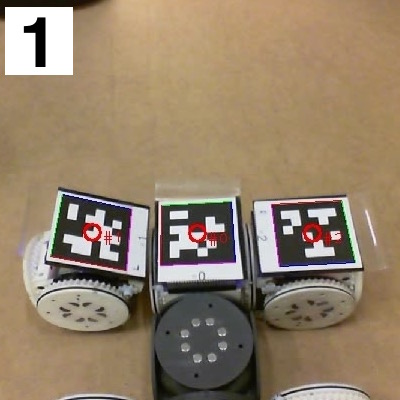
\includegraphics[width=\textwidth]{images/reconf_detach.jpg}
        \label{fig:reconfa}
        \caption{Module detaches from the rest of the robot}
    \end{subfigure}
    \begin{subfigure}[t]{0.32\columnwidth}
        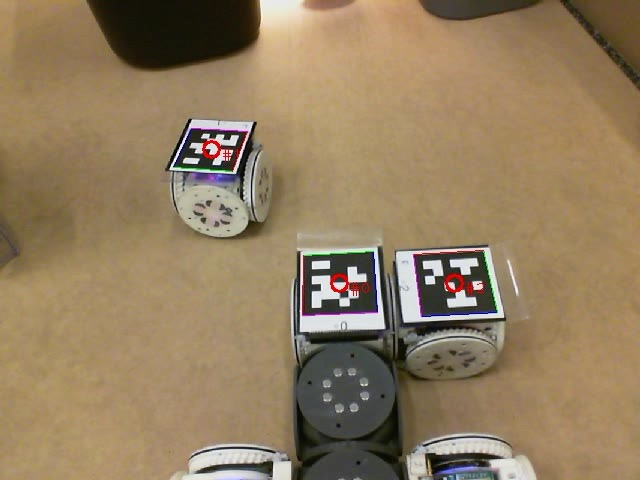
\includegraphics[width=\textwidth]{images/reconf_drive.jpg}
        \label{fig:reconfb}
        \caption{Module drives to the new location}
    \end{subfigure}
    \begin{subfigure}[t]{0.32\columnwidth}
        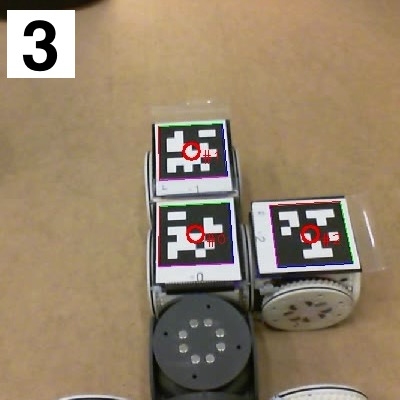
\includegraphics[width=\textwidth]{images/reconf_attach.jpg}
        \label{fig:reconfc}
        \caption{Module attaches to the rest of the robot}
    \end{subfigure}
    \caption{An example of a module operation for reconfiguration.}
      \label{fig:reconf}
\end{figure}

\paragraph{Post-reconfiguration} Once all module movement operations have completed and the goal topology is formed, the robot changes its joint angles to assume a stance in which the goal configuration can begin performing desired behaviors, and if necessary, the robot picks up any objects it dropped. This completes the reconfiguration process. 

\subsection{Comparison with Existing Methods}
Our method of reconfiguration has distinct advantages and disadvantages compared to existing methods.  To the authors' knowledge, use of an onboard overhead camera to provide fiducial-based localization for reconfiguration is novel.  This centralized strategy provides localization only near the sensor module, so the number of modules that can reconfigure simultaneously is limited by the size of the reconfiguration zone.  This means it could not be directly scaled to large clusters of modules the way some existing distributed methods could be (\cite{Yim2007},\cite{Murata2006},\cite{Rubenstein2004}).  However, it is not clear how these distributed methods would be employed in the context of a high-level task.  Additionally, most require one sensor module per distinct cluster, which is cumbersome.

By exploiting high-fidelity centralized localization and the individual mobility of the SMORES-EP modules, we achieve reconfiguration that is rapid, robust, and cleanly deployable in the context of a high-level task.  In our experiments (Section~\ref{sec:experiments}), we observed that the pre-reconfiguration state required about 20 seconds, each module movement operation required about 45 seconds, and post-reconfiguration required about 10 seconds.  Each reconfiguration action had a success rate over 90\%.  This compares very favorably with existing methods, in which each reconfiguration action can take on the order of ten minutes \cite{Yim2007},\cite{Murata2006},\cite{Rubenstein2004}\TODO{Verify exact numbers}.

%     __  ___       __          __                   __
%    / / / (_)___ _/ /_        / /   ___ _   _____  / /
%   / /_/ / / __ `/ __ \______/ /   / _ \ | / / _ \/ /
%  / __  / / /_/ / / / /_____/ /___/  __/ |/ /  __/ /
% /_/ /_/_/\__, /_/ /_/     /_____/\___/|___/\___/_/
%         /____/
%%
\section{High-Level Planner}
\label{sec:high-level}
%
% Automaton
\begin{figure}
\begin{center}
\includegraphics[width=0.4\textwidth]{images/autSimple.png}
\caption{Planner Automaton}
\label{fig:automaton}
\end{center}
\end{figure}

To utilize the sensing and actuation capabilities of the robot as a complete system for accomplishing various tasks, we employ an existing framework called LTLMoP for automatically generating robot controller from user specified high-level instructions using formal method \TODO{cite}.
LTLMoP allows us to use each component of our system as a low-level atomic controller and specify a wide-range of reactive robotic tasks as a set of high-level instructions using these controllers.
We direct readers to \TODO{cite} for more details on LTLMoP.
In this section, we will mainly discuss how we model our system in order to use LTLMoP to automatically generate a high-level controller for our desired robot task.

\subsection{Synthesize a controller}
We first abstract our system and the environment with a set of Boolean propositions.
A system proposition ``pickUp'' is \lt means that the robot is picking up an item and \lf otherwise.
An environment proposition ``pinkObject'' is \lt means that the robot is currently sensing a pink object and \lf otherwise.
Then we can specify the robot task in high-level instructions, such as Structured English, supported by LTLMoP.
Spec.~\ref{spec:simple} is an example of a robot task written in Structured English for searching a pink object and picking it up once the robot finds it.
\begin{spec}[h!]
\caption{Search and pick up a pink object}
\label{spec:simple}
\vspace{-0.1cm}
\small\setlength{\jot}{0pt}
\begin{fleqn}[3pt]
\leqnomode
\begin{subequations}
\renewcommand{\theequation}{\arabic{equation}} 
\makeatletter
\renewcommand\tagform@[1]{\maketag@@@{\ignorespaces#1\unskip\@@italiccorr}}
\makeatother
\hskip-10cm
\begin{alignat}{2}
&\text{do {\bf explore} if and only if you are not sensing {\bf pinkObject}}&& \notag \\ 
&\hspace{1cm}\text{and you are not activating {\bf pickUp}}&& \notag \\
& \text{do {\bf driveToObject} if and only if you are not activating {\bf pickUp}}&& \notag \\
&\hspace{1cm} \text{and you are sensing {\bf pinkObject}}&& \notag \\
& \text{do {\bf pickUp} if and only if you were activating {\bf driveToObject}} && \notag \\
&\hspace{1cm} \text{and you are sensing {\bf arrived}} &&  \notag
\end{alignat}
\end{subequations}
\end{fleqn}
\vspace{-0.4cm}
\end{spec}

In additions to ``pickUp'' and ``pinkObject'', there are some more propositions. 
``explore'' and ``driveToObject'' are system propositions that each represents a different robot action.
``arrived'' is an environment proposition that is \lt if the robot arrives at the pink object.

Using LTLMoP, we can synthesize a robot controller, if one exists, that satisfies the given robot task. The controller is in the form of a finite state automaton as shown in Fig.~\ref{fig:automaton}. Each state is labeled with the value of all system propositions. We denote a proposition with the value of \lf using a ``!'' prefix. Each transition between two states is labeled with the value of {\tt some} environment propositions. Some states and transitions are omitted for clear presentation.

\subsection{Execute a controller}
Since the synthesized high-level controller is a discrete finite state automaton, we need to implement it continuously in order to control the robot to satisfy the given task. 
Each system proposition is mapped to a low-level control program that commands the robot to perform some behaviors.
For example, the proposition ``pickUp'' is mapped to a program that will be executed when ``pickUp'' is \ltnsp. The program command the robot to perform a predefined behavior that will pick up a small magnetic object in front of the robot.
Each environment propositions is mapped to a low-level sensing program that gathers and processes the information from sensors in order to characterize the environment state.
For example, the propositions ``pinkObject'' is mapped to a sensing program that returns \lt or \lf based on whether the robot can detect a predefined pink object with its camera.

To execute the synthesized high-level controller, we start with the predefined initial state in the finite state automaton.
In each iteration, first we determine the value of each environment propositions by calling each corresponding sensing program.
We then can find the next state in the finite state automaton by taking the transition that matches with the current values of all environment propositions.
At last, we execute the corresponding control program based on the value of each system proposition specified in the next state and continue to the next iteration.
For example, we start in the top state in Fig.~\ref{fig:automaton} and execute the ``explore'' program.
If the robot senses a pink object, the value of ``pinkObject'' is \lt and therefore the next state is the bottom right state. We then stop the ``explore'' program and execute the ``driveToObject'' program.

%     ______                     _                      __
%    / ____/  ______  ___  _____(_)___ ___  ___  ____  / /______
%   / __/ | |/_/ __ \/ _ \/ ___/ / __ `__ \/ _ \/ __ \/ __/ ___/
%  / /____>  </ /_/ /  __/ /  / / / / / / /  __/ / / / /_(__  )
% /_____/_/|_/ .___/\___/_/  /_/_/ /_/ /_/\___/_/ /_/\__/____/
%           /_/
\section{Experiment Results}
\label{sec:experiments}
%

To validate and demonstrate the capabilities of our system, an experiment was run in which a robot composed of SMORES-EP modules completed a complex, high-level task in an unknown environment. Figure \ref{fig:map} shows the environment layout, designed to represent a cluttered office. The high-level task consisted of 5 sub-tasks of 3 different types: explore the environment, find and retrieve 2 objects in the office, and deliver each to a drop-off zone. One object was in the open (a ``free'' environment type), and the other was positioned between two obstacles (a ``tunnel'' environment). Obstacles, environment types, and locations of the objects and drop-off zone were unknown to the robot \textit{a priori}.
Spec.~\ref{spec:experiment} shows the high-level instructions from the user for synthesizing a robot controller for this experiment.

5 SMORES-EP modules, 1 Sensor Module, and 3 dummy modules were used to compose the robot for performing the task. Steel objects were attached to and carried using the electro-permanent magnets of the SMORES-EP modules.
The two configurations and five behaviors described in Section \ref{sec:configuration-specifics} were available for selection by the high-level planner for this experiment.


% Map
\begin{figure}
\begin{center}
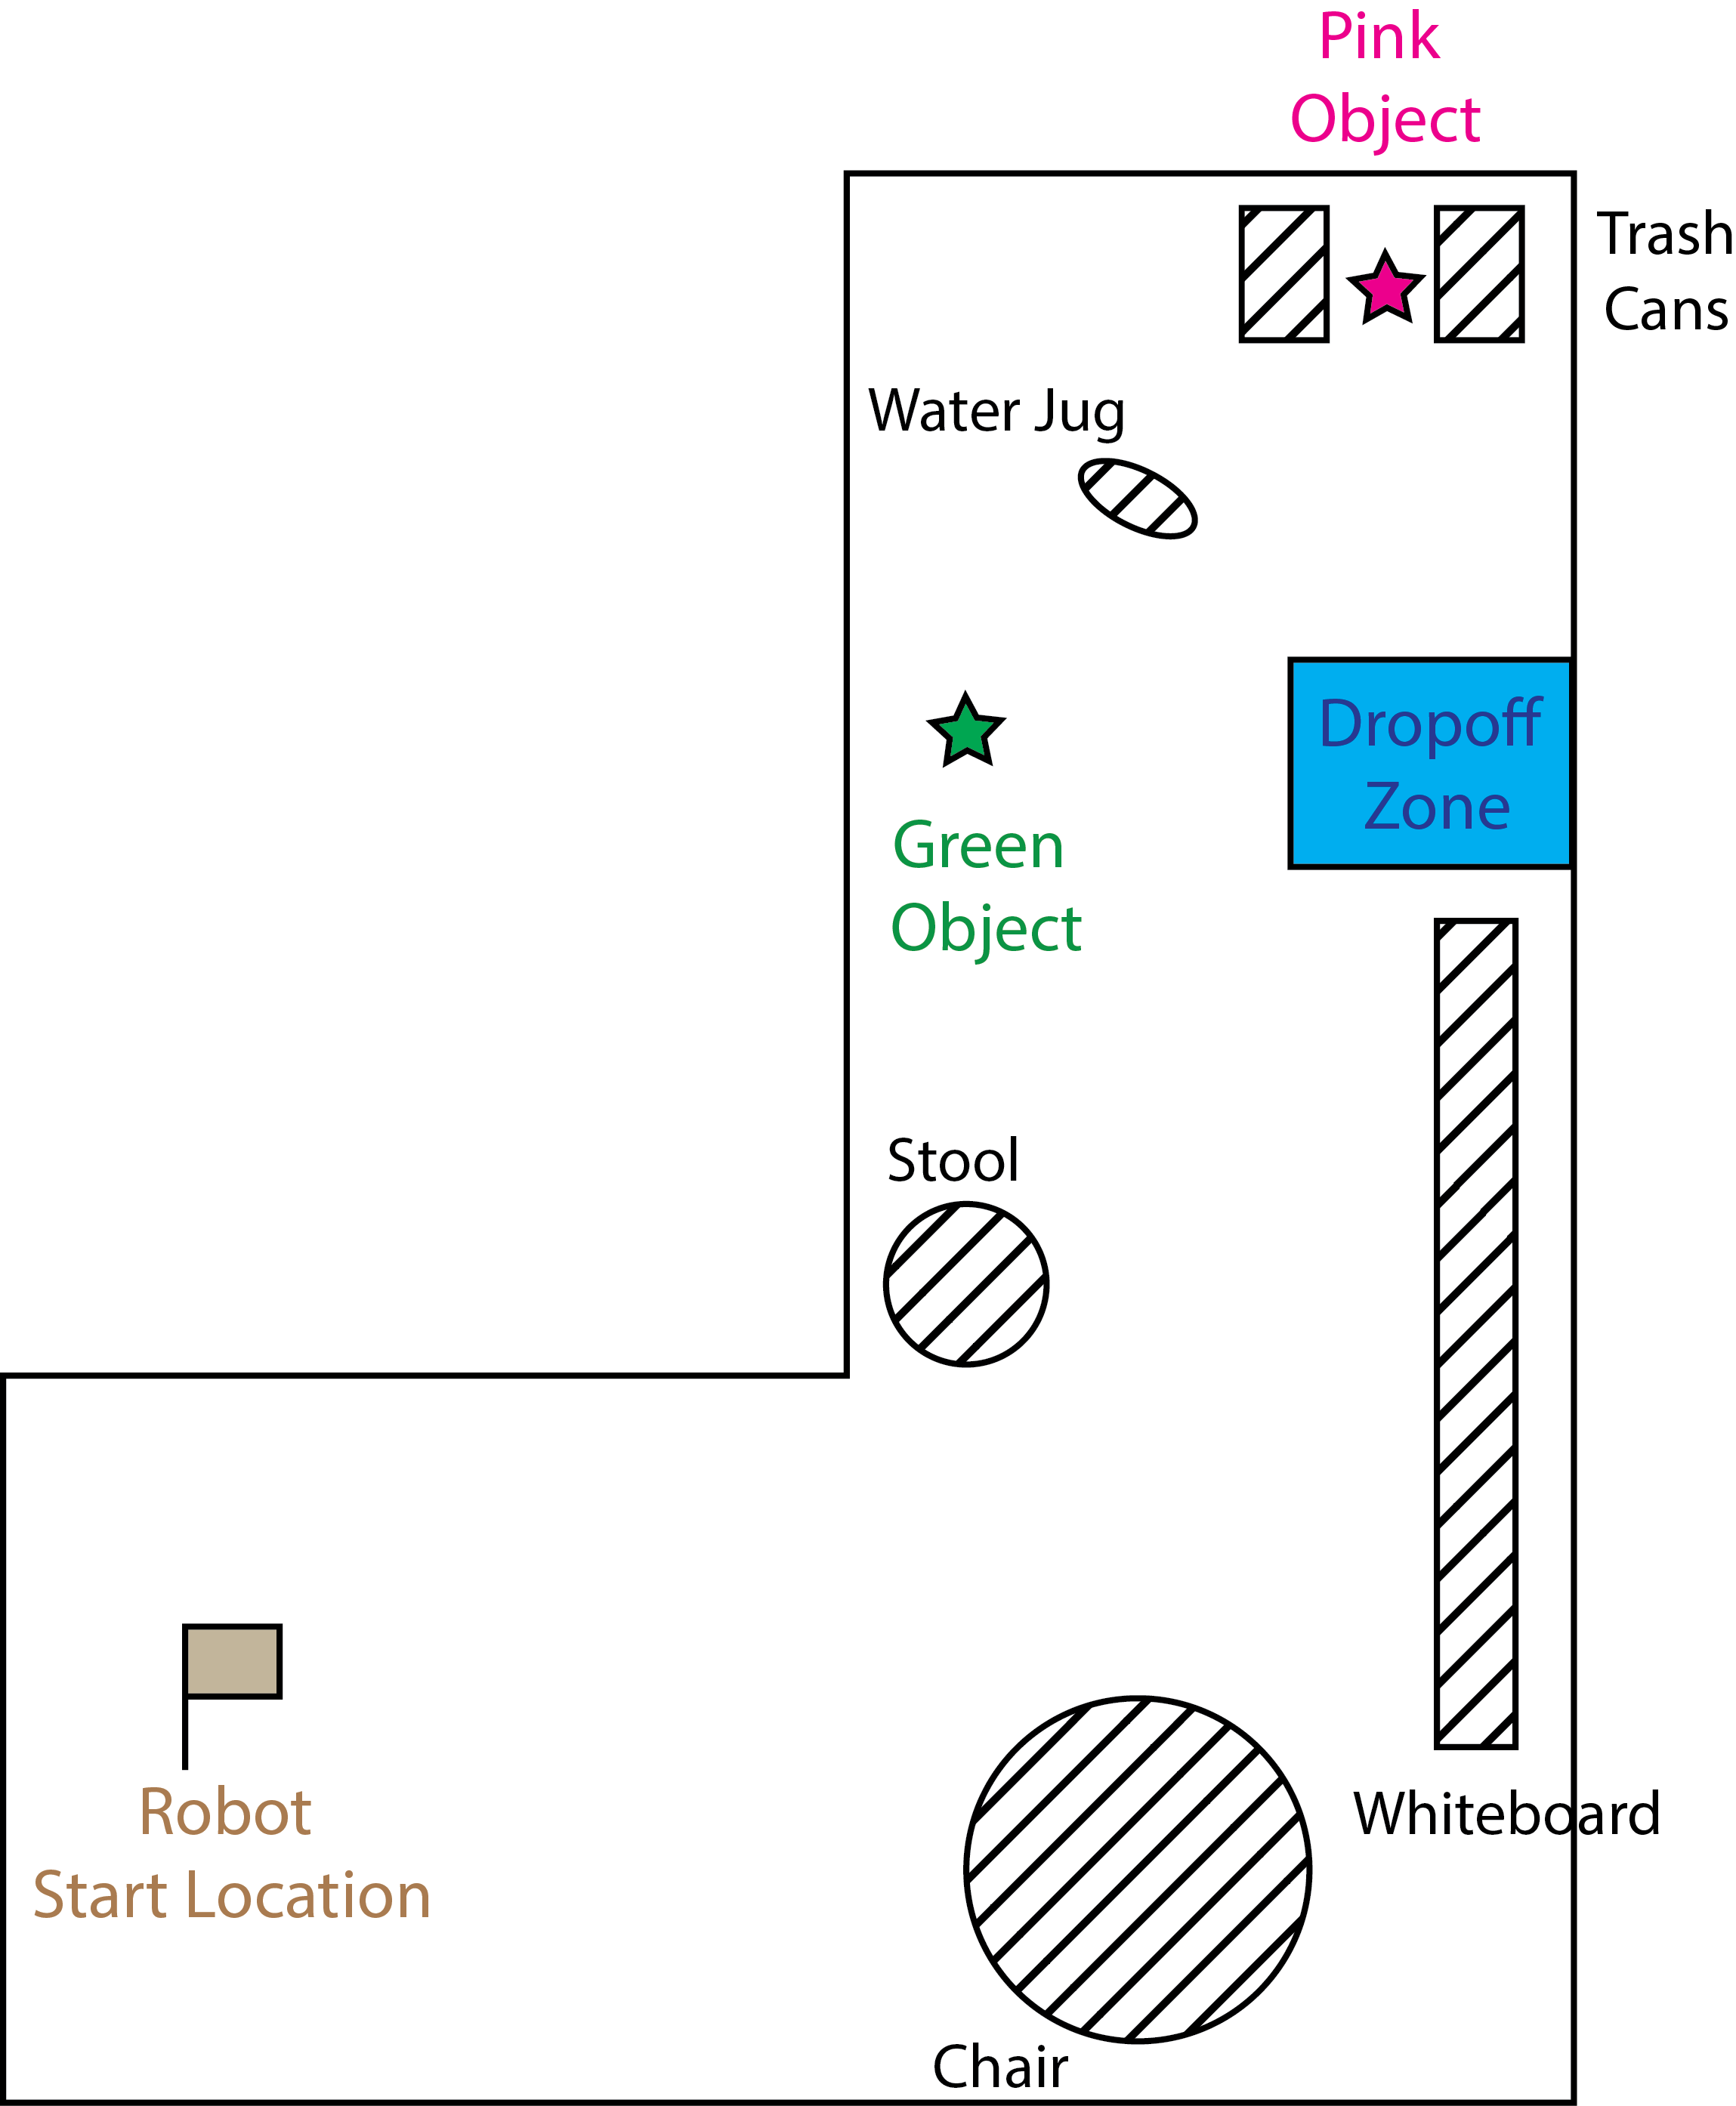
\includegraphics[width=0.4\textwidth]{images/RSSMap.png}
\caption{Diagram of experiment environment}
\label{fig:map}
\end{center}
\end{figure}

\begin{figure*}[t]
      \centering
      \begin{subfigure}[t]{0.32\textwidth}
        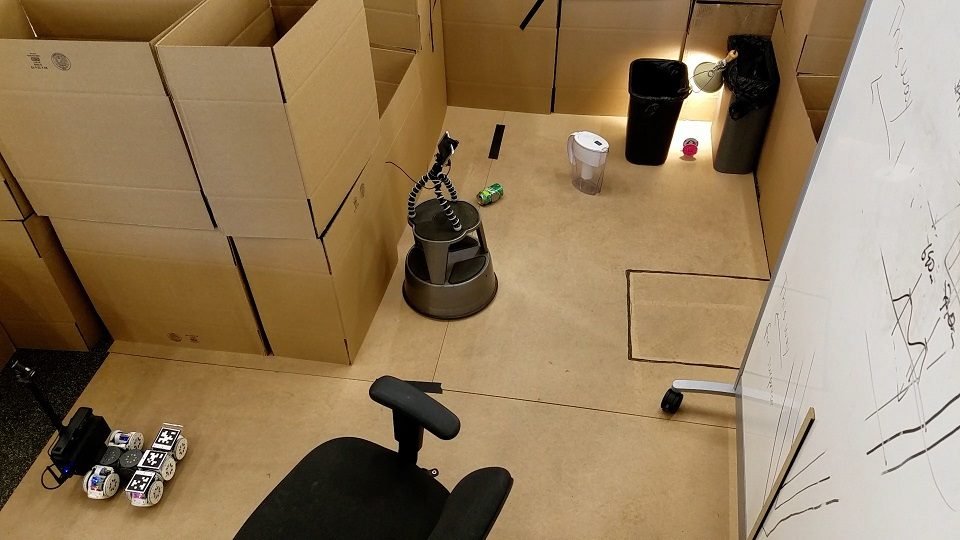
\includegraphics[width=\textwidth]{images/overhead_starting.jpg}
        %\label{fig:obja}
        \caption{Experiment setup and robot starting location}
    \end{subfigure}
    \begin{subfigure}[t]{0.32\textwidth}
        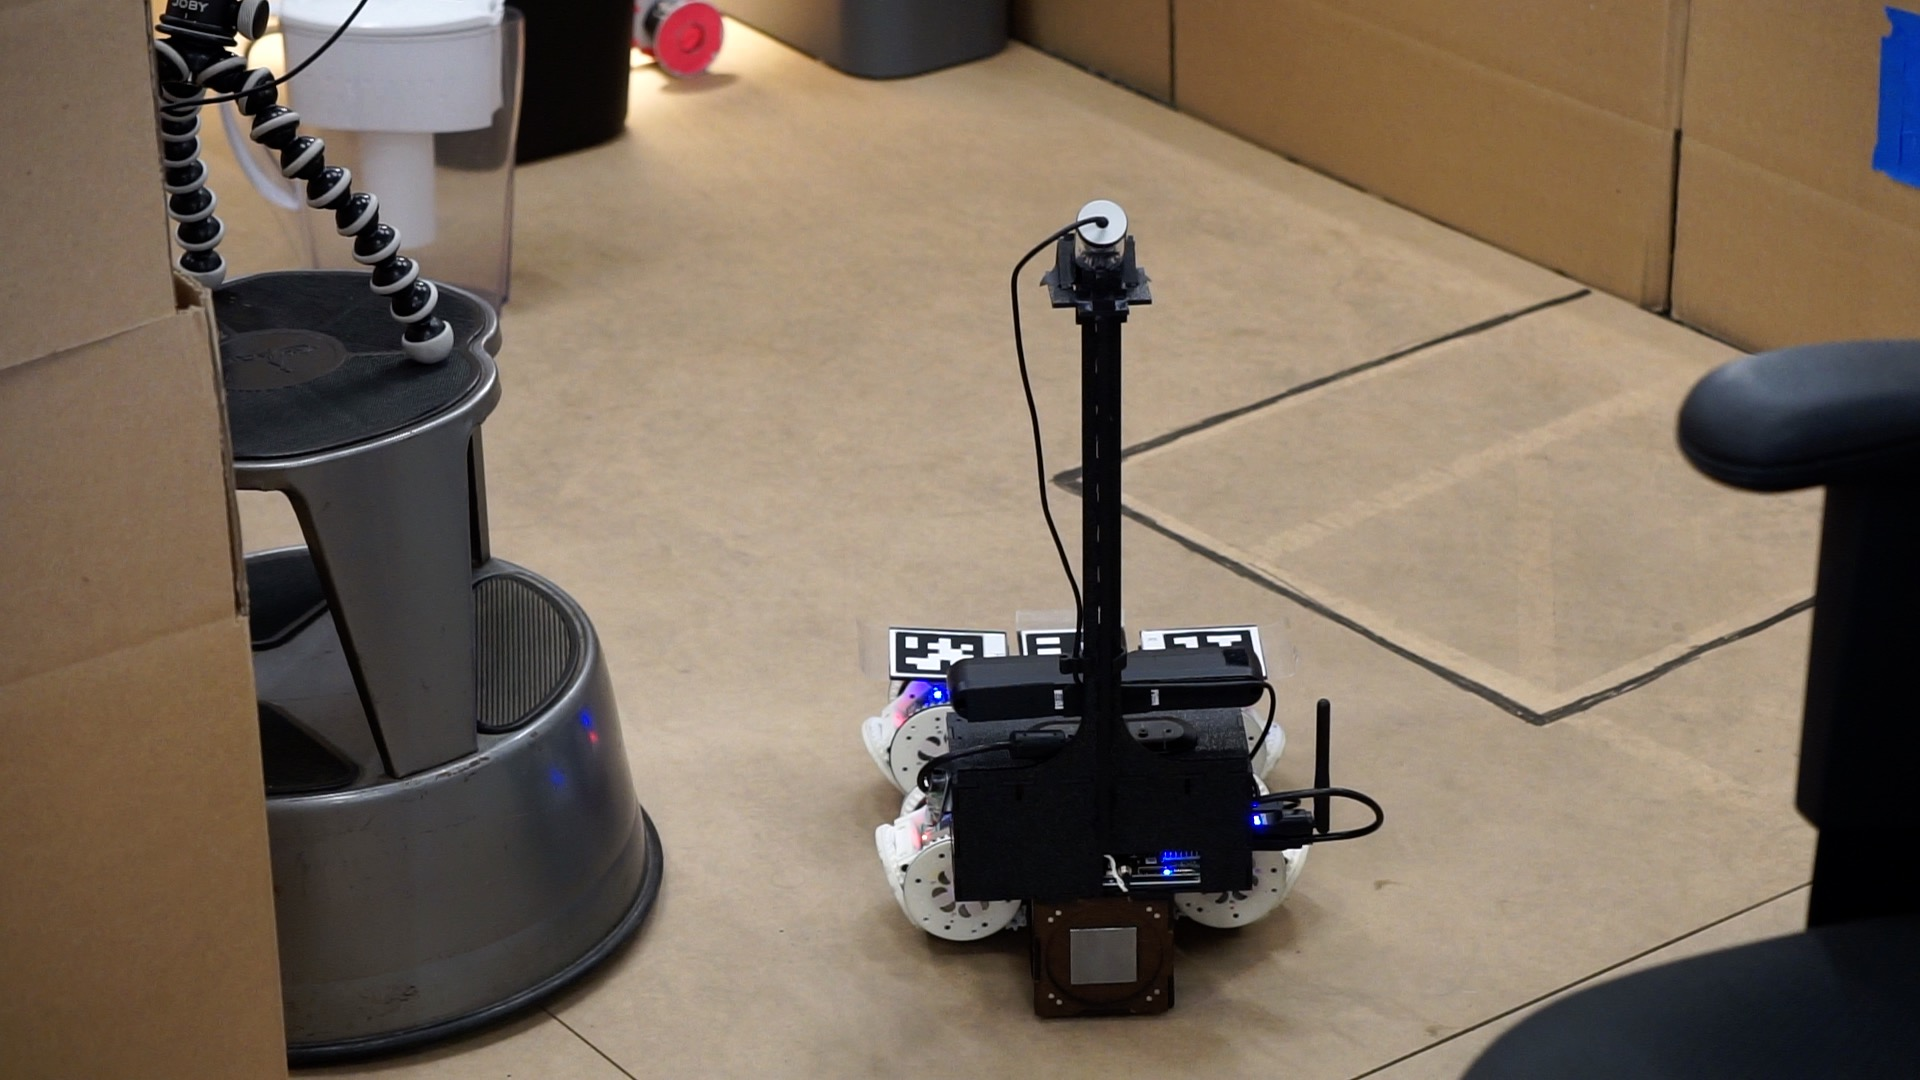
\includegraphics[width=\textwidth]{images/exploration.jpg}
        %\label{fig:objb}
        \caption{Exploring environment while searching for objects}
    \end{subfigure}
    \begin{subfigure}[t]{0.32\textwidth}
        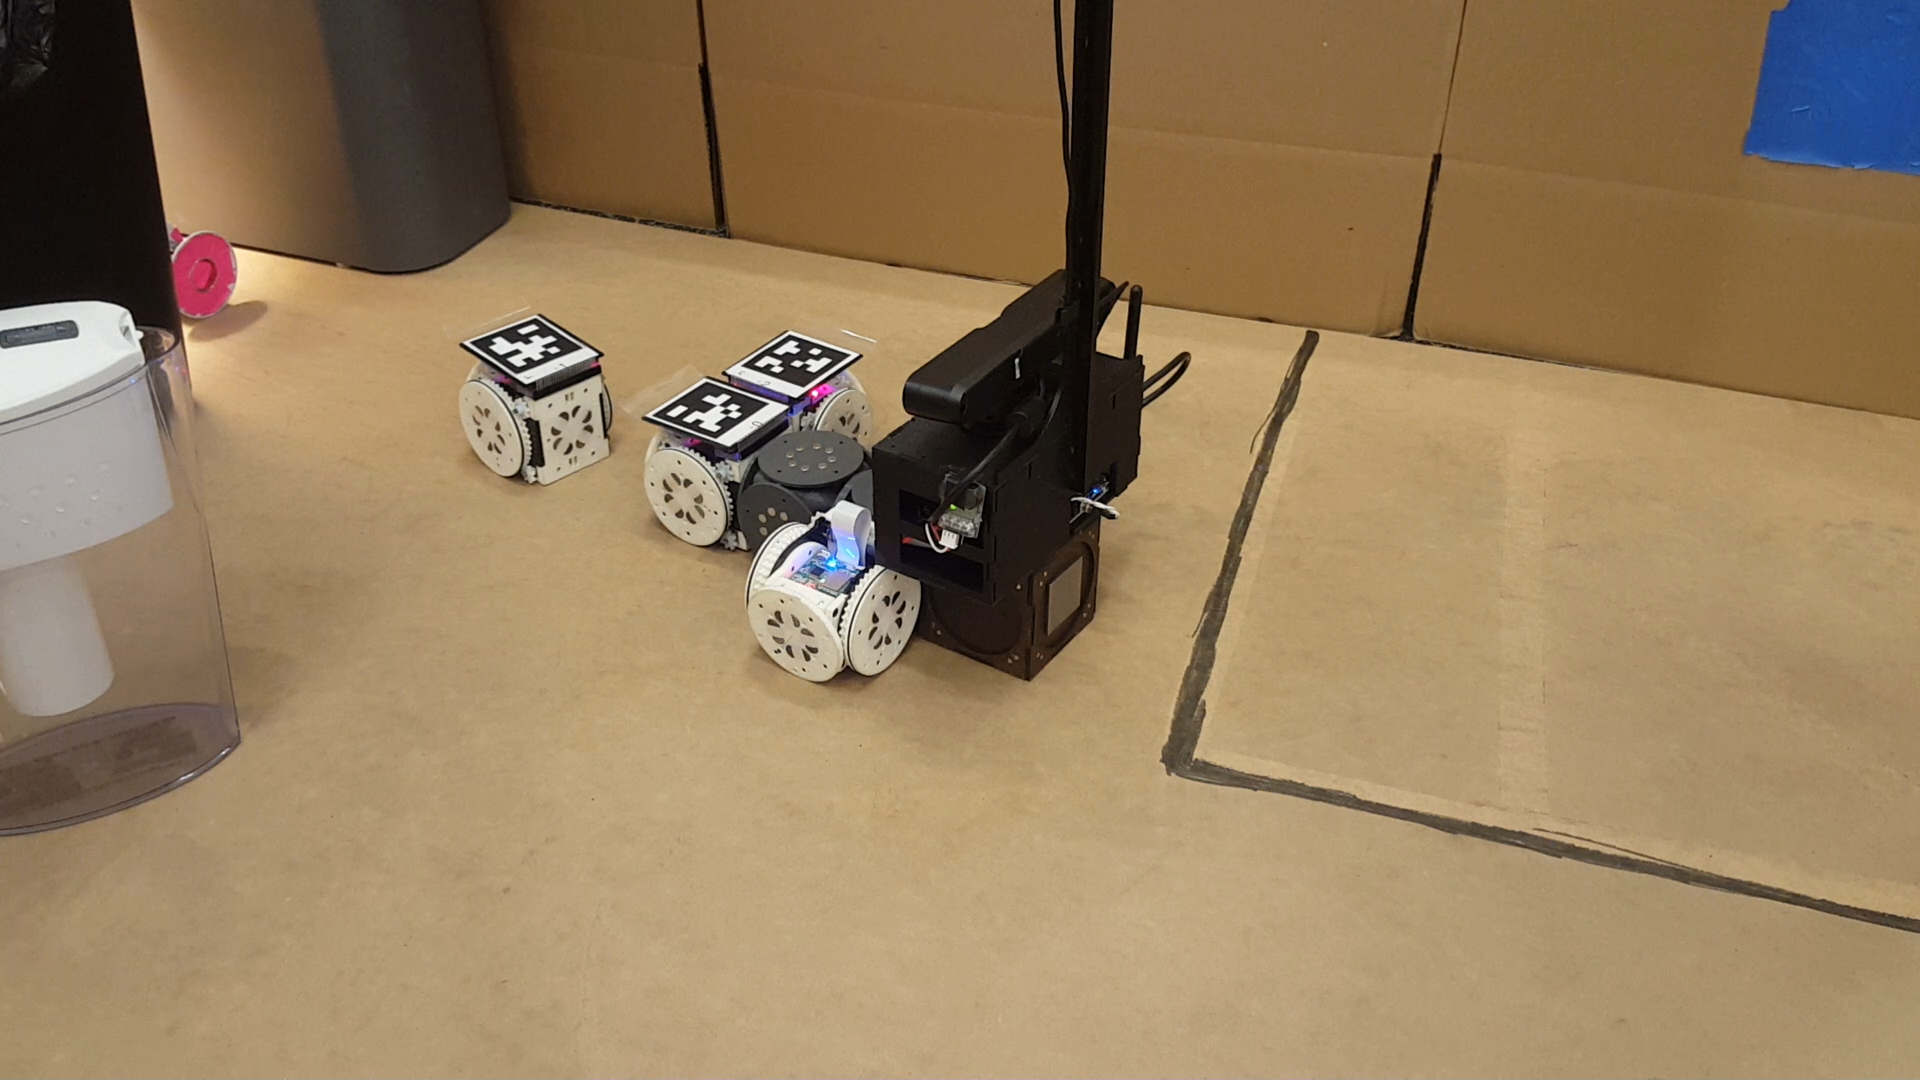
\includegraphics[width=\textwidth]{images/reconfiguration.png}
        %\label{fig:objb}
        \caption{Reconfiguring to retrieve pink object}
    \end{subfigure}
    \begin{subfigure}[t]{0.32\textwidth}
        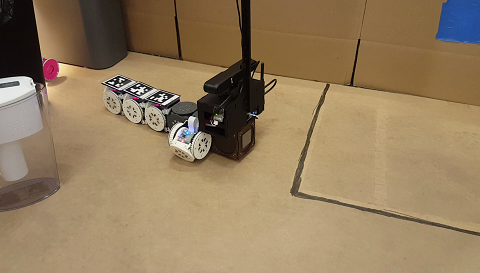
\includegraphics[width=\textwidth]{images/pink_retrieval.png}
        \caption{Retrieving pink object}
        \label{fig:pink_grab}
    \end{subfigure}
    \begin{subfigure}[t]{0.32\textwidth}
        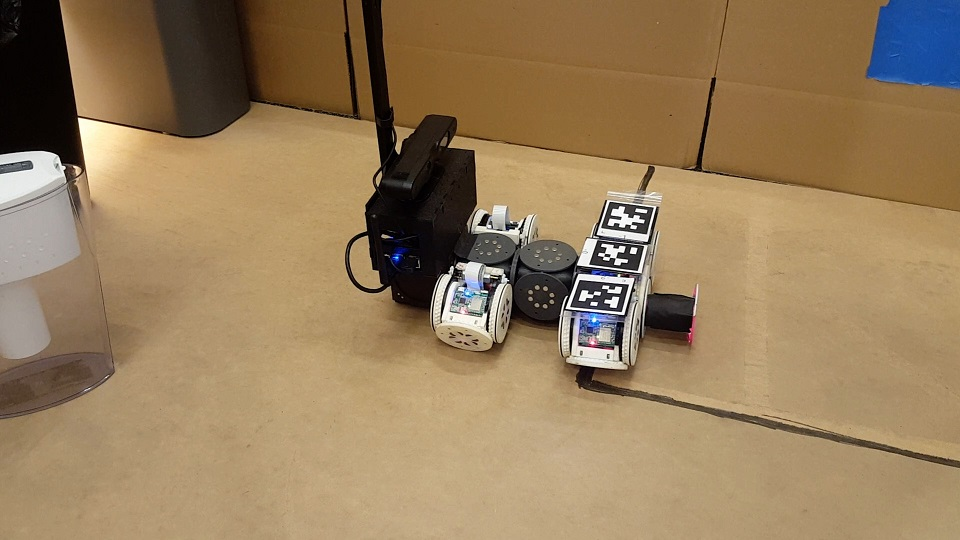
\includegraphics[width=\textwidth]{images/dropoff.jpg}
        \caption{Dropping off an object in the delivery zone}
        \label{fig:dropoff}
    \end{subfigure}
    \begin{subfigure}[t]{0.32\textwidth}
        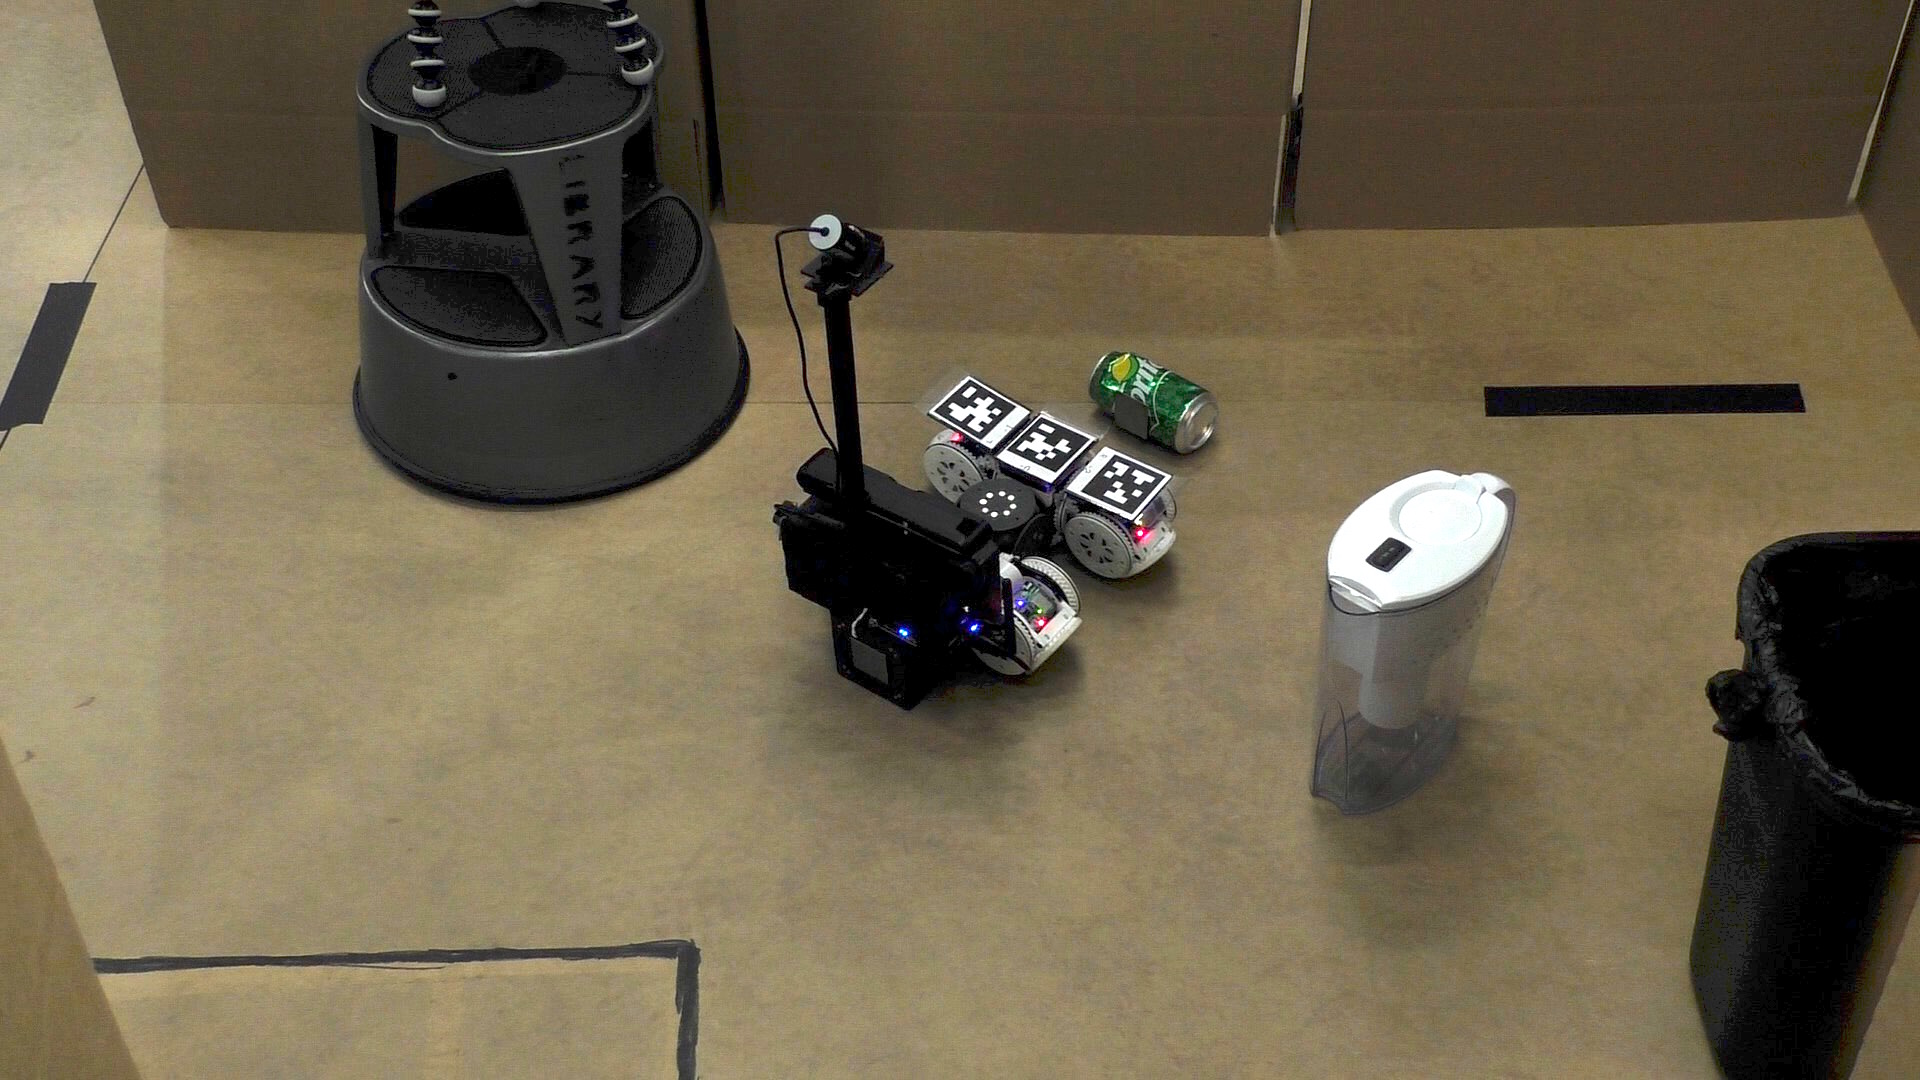
\includegraphics[width=\textwidth]{images/green_retrieval.jpg}
        %\label{fig:objb}
        \caption{Retrieving green object}
    \end{subfigure}
      \caption{Environment characterization types for object retrieval.}
      \label{fig:demo}
   \end{figure*}

\begin{spec}[h!]
\caption{Search and move any pink or green object to the drop-off zone}
\label{spec:experiment}
\vspace{-0.1cm}
\small\setlength{\jot}{0pt}
\begin{fleqn}[3pt]
\leqnomode
\begin{subequations}
\renewcommand{\theequation}{\arabic{equation}} 
\makeatletter
\renewcommand\tagform@[1]{\maketag@@@{\ignorespaces#1\unskip\@@italiccorr}}
\makeatother
\hskip-10cm
\begin{alignat}{2}
&\text{ {\bf carry} is set on {\bf pickup} and reset on {\bf drop}}&& \notag \\
&\text{if you are not activating ({\bf carry} or {\bf pickup} or {\bf drop}}&& \notag \\
&\hspace{1cm}\text{or {\bf driveToItem} or {\bf driveToDropoff}) then do {\bf explore}}&& \notag \\
&\text{if you are activating {\bf carry} and you are not sensing {\bf dropoffzone}}&& \notag \\
&\hspace{1cm}\text{then do {\bf explore}}&& \notag \\
&\text{do {\bf driveToDropoff} if and only if you are activating {\bf carry} }&& \notag \\
&\hspace{1cm}\text{and you are sensing {\bf dropoffzone}}&& \notag \\
&\text{do {\bf driveToItem} if and only if you are not activating {\bf carry} }&& \notag \\
&\hspace{1cm}\text{and you are sensing {\bf item}}&& \notag \\
&\text{do {\bf drop} if and only if you were activating {\bf driveToDropoff } }&& \notag \\
&\hspace{1cm}\text{and you are sensing {\bf arrived}}&& \notag \\
&\text{do {\bf pickup } if and only if you were activating {\bf driveToItem  } }&& \notag \\
&\hspace{1cm}\text{and you are sensing {\bf arrived}}&& \notag \\
&\text{infinitely often not {\bf carry}}&& \notag
\end{alignat}
\end{subequations}
\end{fleqn}
\vspace{-0.4cm}
\end{spec}


Figure \ref{fig:demo} shows snapshots from the experiment run. A video of the entire experiment is available as an attachment to this paper. The starting location prevented the robot from seeing the objects initially, forcing it to explore the environment to search for them. After a period of exploration the robot discovered the pink object first. The characterization algorithm correctly classified the surrounding environment as a ``tunnel'' type, and accordingly the robot navigated in front of the object and reconfigured to the ``proboscis'' configuration. Once this was done, the object was retrieved and pulled out into the open. The robot then dropped the object, reconfigured back to the ``car'' configuration for navigation to the drop-off zone, and again retrieved the object. The robot then navigated to and dropped off the object at the drop-off zone, which was seen during exploration and recorded in the global map built by the SLAM algorithm. Once done, the robot navigated to the green object which was correctly determined to not require any reconfiguration. No further exploration was required since the green object was discovered while the robot was dropping off the pink object. The robot finished the experiment by also delivering the green object to the drop-off zone. Figure \ref{fig:octomap} shows the final volumetric map of the environment explored by the robot as it explored the environment and delivered objects. The robot successfully completed all tasks in the experiment in about 26 minutes. Note that the video shows a human reaching into the field to touch the green object once the robot comes into contact with it. This was due to a error on the field resulting in the object becoming stuck between two floor boards, so a human dislodged it so the robot could grasp it normally.


\begin{figure}
\begin{center}
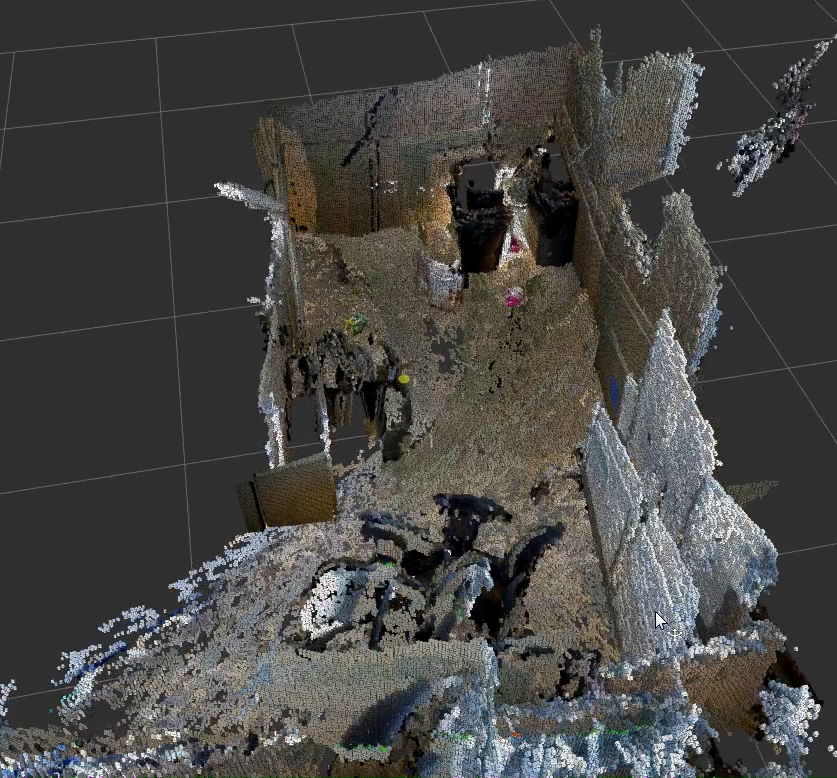
\includegraphics[width=0.45\textwidth]{images/octomap.png}
\caption{Volumetric map of environment built by visual SLAM}
\label{fig:octomap}
\end{center}
\end{figure}

%     ____  _                           _
%    / __ \(_)___________  ____________(_)___  ____
%   / / / / / ___/ ___/ / / / ___/ ___/ / __ \/ __ \
%  / /_/ / (__  ) /__/ /_/ (__  |__  ) / /_/ / / / /
% /_____/_/____/\___/\__,_/____/____/_/\____/_/ /_/
\section{Discussion}
\label{sec:discussion}
%
\subsection{Challenges}
The experiment demonstrated that our system can autonomously perform complex high-level tasks in an unknown environment. It also revealed many issues that make autonomous reactive tasks difficult to achieve in modular systems. This section discusses issues that were observed and solutions that were implemented to overcome them.

Due to limitations of individual modules, robot speed was very low. In addition, having a robotic system composed of 6 individual robotic components (5 SMORES-EP modules and 1 sensor module) multiplies the chance of a component having a hardware failure. The long runtime combined with multiplied failure points resulted in a high risk of an error occurring during the experiment. Thus, each system component had to be designed with features to make it as robust as possible, and several error recovery features had to be implemented in the system.

The processing power required for perception and environment characterization presented issues with size and computation speed. As can be seen from Figure~\ref{fig:sensor-module}, the sensor module is significantly larger than a regular module in order to hold the required sensors and computer board. This imposes significant limitations on possible configurations and their locomotion abilities, due to the low connection strength and power of modules. At the same time, the small computer board used in the sensor module results in low computation power, which causes the sensor processing and perception algorithms to run slowly and have less accuracy. Simple configuration designs and efficient algorithms were used to address these issues. Future autonomous modular systems would benefit significantly from powerful but highly compact, lightweight sensing and processing components that can be carried onboard the robot while imposing minimal size and weight constraints.

As with many autonomous systems, uncertainties such as sensor noise and controller lag create issues with robust behavior. For example, the global map and robot pose determined by visual SLAM accumulate significant errors (due to sensor noise) as time progresses. To compensate, repetitive feedback controllers and checks were implemented during task performance. As the robot navigates toward and retrieves objects, it constantly updates its estimate of the object location as new measurements of the object are received. During reconfiguration, docking modules are checked and re-aligned several times during the docking process to ensure they are lined up precisely before connecting to each other. This helps the robot recover from controller lag or noisy AprilTag measurements.

Finally, some simple hardware failures were encountered during experiment runs. Since SMORES-EP modules are research prototypes built from scratch, they are more prone to failures such as microcontroller errors and position control errors from custom encoders. Future experiments can be improved in robustness by improving the hardware quality of modules to bring them closer to the level of a commercial product.
%
\subsection{Future Work and Conclusion}
%
We presented a novel system for autonomously accomplishing high-level tasks in unknown environments with modular self-reconfigurable robots.  This system is the first to use perception of an unknown environment to reactively perform complex high-level tasks using intelligent reconfiguration. Components of this system include novel controller synthesis, environment characterization, and self-reconfiguration methods. The system was validated using a physical experiment using a high-level task consisting of a heterogenous set of 5 sub-tasks in an \textit{a priori} unknown environment. 

The system is not without limitations, and could be significantly extended in future work.  First and foremost, the experiment we present utilizes only two configurations, and our perception system demonstrates the ability to recognize only two special environments (ledge and tunnel).  MSRR systems are supposed to provide wide flexibility at addressing tasks. To truly prove this promise, we need to demonstrate that MSRR systems can reconfigure between a much wider variety of morphologies, in response to a large number of environments.  We believe that our system could be extended to such scenarios, but we do not minimize the difficulty of the problems one should expect to encounter in tackling these problems. 

While the presented system successfully demonstrated that modular robots can autonomously achieve a realistic object retrieval task, limitations of the modular hardware make them unsuitable for application in harsh real-world scenarios such as search-and-rescue.  One of the biggest limitations is simply the small size and small forces that can be applied by the modules.  Given current actuator and connector technology, it is still very difficult to apply large enough forces to operate in a realistic search-and-rescue environment. 

It is important to consider how the presented system could be adapted to work with other modular robot hardware.  Certain aspects of the system are almost entirely hardware-independent, such as the sensing and navigation tools, the high-level planner, and the hardware abstractions.  The reconfiguration method is in some ways specific to SMORES-EP, because it relies on the ability of each module to move by differential drive on the flat plane.  The majority of MSRR hardware systems do not have this capability, and would not be able to reconfigure in this way.  However, we believe the success of this novel reconfiguration method could have some implications for MSRR hardware design: future designers might want to consider designing for individual motility and forgiving connectors, in order to take advantage of a reconfiguration method similar to the one present.

To conclude, this paper presents the first system that enables modular self-reconfigurable robots to autonomously achieve tasks requiring perception-informed reconfiguration in an unknown environment.  This capability is crucial to the success of modular robots as a technology, and by demonstrating it for the first time, we believe we have taken a real step toward the application of modular robots to solve tasks in the real world.
%
\section*{Acknowledgments}
%
This work was funded by NSF grant numbers CNS-1329620 and CNS-1329692.


       %     ____       ____
       %    / __ \___  / __/__  ________  ____  ________  _____
       %   / /_/ / _ \/ /_/ _ \/ ___/ _ \/ __ \/ ___/ _ \/ ___/
       %  / _, _/  __/ __/  __/ /  /  __/ / / / /__/  __(__  )
       % /_/ |_|\___/_/  \___/_/   \___/_/ /_/\___/\___/____/

%% Use plainnat to work nicely with natbib. 
\bibliographystyle{plainnat}
\bibliography{references}

\end{document}



















